%%%%%%%%%%%%%%%%%%%%%%%%%%%%%%%%%%%%%%%%%%%%%%%%%%%%%%%%%%%%%%%%%%%%%%%%%%%%%%%%
%2345678901234567890123456789012345678901234567890123456789012345678901234567890
%        1         2         3         4         5         6         7         8

%\documentclass[letterpaper, 10 pt, conference]{ieeeconf}  % Comment this line out
                                                          % if you need a4paper
\documentclass[a4paper, 10pt, conference]{llncs}      % Use this line for a41
                                                          % paper

\usepackage{amsmath}
\usepackage{epsf,graphicx,subfig}
\setcounter{tocdepth}{3}
\usepackage{color}
\usepackage{lineno}
\usepackage[nolist]{acronym}
\usepackage{epsf,graphicx,subfig}
\usepackage{amssymb,amsmath}
\usepackage{tikz}
\usetikzlibrary{positioning}
\usepackage{todonotes}
\usepackage{standalone}
\usepackage{scalefnt}
\usepackage{url}
%\urldef{\mailsa}\path|{jmassich,joanm,|
%\urldef{\mailsb}\path|anna.kramer, leonie.kunz, christine.reiss, nicole.sator,|
%\urldef{\mailsc}\path|erika.siebert-cole, peter.strasser, lncs}@eia.udg.edu|    
\newcommand{\keywords}[1]{\par\addvspace\baselineskip
\noindent\keywordname\enspace\ignorespaces#1}

% See the \addtolength command later in the file to balance the column lengths
% on the last page of the document

\title{\acs{sift} texture description for understanding breast ultrasound images}
\author{Joan Massich\inst{1}\inst{2}\thanks{This work was partially supported by the Spanish Science and Innovation grant nb. TIN2012-37171-C02-01 and TTIN2012-37171-C02-02 and the Regional Council of Burgundy.} \and Fabrice Meriaudeau \inst{2} \and Melcior Sent{\'i}s\inst{3} \and Sergi Ganau\inst{3} \and Elsa~P{\'e}rez\inst{4} 
\and Domenec Puig\inst{5} \and Robert  Mart{\'i} \inst{1} \and  Arnau Oliver\inst{1}\and Joan Mart{\'i} \inst{1}}
\institute{Computer Vision and Robotics Group, University of Girona, Spain. \email{jmassich@atc.udg.edu} \and
Laboratoire Le2i-UMR CNRS, University of Burgundy,  Le Creusot, France.
 \and Department of
Breast and Gynecological Radiology,  UDIAT-Diagnostic Center, Parc
Taul{\'i} Corporation, Sabadell, Spain.
 \and 
Department of Radiology, Hospital Josep Trueta of Girona, Spain.
\and
Department of Computer Engineering and Mathematics, University Rovira i Virgili, Tarragona, Spain.}
%\author{}

\begin{document}

\frontmatter
\pagestyle{empty}

\mainmatter  % start of an individual contribution

% The following packages can be found on http:\\www.ctan.org
%\usepackage{graphics} % for pdf, bitmapped graphics files
%\usepackage{epsfig} % for postscript graphics files
%\usepackage{mathptmx} % assumes new font selection scheme installed
%\usepackage{times} % assumes new font selection scheme installed
%\usepackage{amsmath} % assumes amsmath package installed
%\usepackage{amssymb}  % assumes amsmath package installed




%

%\institute{Computer Vision and Robotics Group, University of Girona, Spain, \email{jmassich@atc.udg.edu}, \and University of Burgundy, Le2i Laboratory CNRS UMR 5158, Esplanade Erasme, 21000, Dijon, France  \and  Dept of Radiology, Hospital Josep Trueta of Girona, Spain.}
 %\and
% Department of Computer Science,  University of Anonymous2, USA.
 %{We are thankful to XYZ}


\maketitle


%\author{Joan Massich i Vall % <-this % stops a space
%\thanks{This work was partially supported by the Spanish Government MEC grant nb. TIN2007-60553, the University of Girona, and  Conseil de Bourgogne.}
%\thanks{Computer Vision and Robotics Group, University of Girona, Catalonia, Spain } \newline
%        {\tt\small jmassich@eia.udg.edu}%
%%%\thanks{P. Misra is with the Department of Electrical Engineering, Wright State University,
%% %       Dayton, OH 45435, USA
%%  %      {\tt\small pmisra@cs.wright.edu}}%
%%%University Hospital Dr Josep Trueta
%%%
%%%
%%%Department of Radiology, Hospital Josep Trueta of Girona, Catalonia, Spain 
%}

%\begin{document}
\begin{acronym}
\acro{gldm}[GLDM]{Gray-Level Difference Method}
\acro{abus}[ABUS]{Automated whole Breast Ultra-Sound}
\acro{acm}[ACM]{Active Contour Model}
\acro{acr}[ACR]{American College of Radiology}
\acro{acwe}[ACWE]{Active Contour Without Edges}
\acro{adf}[ADF]{Anisotropic Diffusion Filter}
\acro{amed}[AMED]{Average Minimum Euclidian Distance}
\acro{aov}[AOV]{Area Overlap}
\acro{ard}[ARD]{Average Radial Derivative}
\acro{are}[ARE]{Average Radial Error}
\acro{birads}[BI-RADS]{Breast Imaging-Reporting and Data System}
\acro{bof}[BoF]{Bag-of-Features}
\acro{bow}[BoW]{Bag-of-Words}
\acro{bus}[BUS]{Breast Ultra-Sound}
\acro{cad}[CAD]{Computer Aided Diagnosis}
\acro{cade}[CADe]{Computer Aided Detection}
\acro{cadx}[CADx]{Computer Aided Diagnosis}
\acro{cas}[CAS]{Computer Aided Surgery}
\acro{cc}[CC]{Cranio-Caudal}
\acro{cdf}[CDF]{Cumulative Distribution Function}
\acro{crf}[CRF]{Conditional Random Field}
\acro{ct}[CT]{Computed Tomography}
\acro{cv}[CV]{Computer Vision}
\acro{dic}[DIC]{Ductal Infiltrating Carcinoma}
\acro{dicom}[DICOM]{Digital Imaging and Communications in Medicine}
\acro{dm}[DM]{Digital Mammography}
\acro{dpm}[DPM]{Deformable Part Model}
\acro{dsc}[DSC]{Dice Similarity Coefficient}
\acro{em}[EM]{Expectation Maximization}
\acro{ffdm}[FFDM]{Full-Field Digital Mammography}
\acro{fna}[FNA]{Fine Needle Aspiration}
\acro{fn}[FN]{False Negative}
\acro{fnr}[FNR]{False-Negative Ratio}
\acro{fp}[FP]{False Positive}
\acro{fpr2}[FPR]{False-Positive Ratio}
\acro{fpr}[FPR']{False-Positive Ratio'}
\acro{gc}[GC]{Graph-Cut}
\acro{gcs}[GCS]{Gaussian Constraining Segmentation}
\acro{glcm}[GLCM]{Gray-Level Co-occurrence Matrix}
\acro{gpb}[gPb]{Global Probability Boundary}
\acro{grasp}[GRASP]{Greedy Randomized Adaptive Search Procedure}
\acro{gt}[GT]{Ground Truth}
\acro{gvf}[GVF]{Gradient Vector Flow}
\acro{hd}[HD]{Hausdorff Distance}
\acro{hgte}[HGTE]{Hidden Ground Truth Estimation}
\acro{hgt}[HGT]{Hidden Ground Truth}
\acro{hog}[HOG]{Histogram of Gradients}
\acro{icm}[ICM]{Iterated Conditional Modes}
\acro{idc}[IDC]{Intra-Ductal Carcinoma}
\acro{iid}[IID]{Independent and Identically Distributed}
\acro{ilc}[ILC]{Infiltrating Lobular Carcinoma}
\acro{itg}[ITG]{Intensity Texture and Geometric}
\acro{jsc}[JSC]{Jaccard Similarity Coefficient}
\acro{lbp}[LBP]{Local Binary Pattern}
\acro{loo}[LOOCV]{Leave-One-Out Cross-Validation} 
\acro{mad}[MAD]{Median Absolute Deviation}
\acro{map}[MAP]{Maximum A Posteriori}
\acro{mcde}[MCDE]{Modified Curvature Diffusion Equation}
\acro{md}[MD]{Minimum Distance}
\acro{ml}[ML]{Maximum Likelihood}
\acro{mlo}[MLO]{Medio-Lateral Oblique}
\acro{mra}[MRA]{Multi Resolution Analysis}
\acro{mrf}[MRF]{Markov Random Field}
\acro{mri}[MRI]{Magnetic Resonance Image}
\acro{nc}[NC]{Normalized Cuts}
\acro{npv}[NPV]{Negative Predictive Value}
\acro{nrv}[NRV]{Normalized Residual Value}
\acro{of}[OF]{Overlap Fraction}
\acro{pca}[PCA]{Principal Component Analysis}
\acro{pde}[PDE]{Partial Differential Equation}
\acro{pdf}[PDF]{Probability Density Function}
\acro{pd}[PD]{Proportional Distance}
\acro{pet}[PET]{Position Emission Tomography}
\acroplural{roi}[ROIs]{ Regions Of Interest}
\acro{ppv}[PPV]{Positive Predictive Value}
\acro{pr}[PR]{Pattern Recognition}
\acro{qc}[QC]{Quadratic-Chi}
\acro{qs}[QS]{Quick-Shift}
\acro{rbf}[RBF]{Radial Basis Function}
\acro{rf}[RF]{Random Forest}
\acro{rgi}[RGI]{Radial Gradien Index}
\acro{rgi}[RGI]{Radial Gradient Index}
\acro{rg}[RG]{Region Growing}
\acro{roi}[ROI]{Region Of Interest}
\acro{sa}[SA]{Simulated Annealing}
\acro{sift}[SIFT]{Self-Invariant Feature Transform}
\acro{si}[SI]{Similarity Index}
\acro{slic}[SLIC]{Simple Linear Iterative Clustering}
\acro{snr}[SNR]{Signal to Noise Ratio}
\acro{som}[SOM]{Self Organizing Map}
\acro{staple}[STAPLE]{Simultaneous Truth and Performance Level Estimation}
\acro{svm}[SVM]{Support Vector Machine}
\acro{tnr}[TNR]{True-Negative Ratio}
\acro{tn}[TN]{True Negative}
\acro{tpr}[TPR]{True-Positive Ratio}
\acro{tp}[TP]{True Positive}
\acro{us}[US]{Ultra-Sound}
\end{acronym}


%\linenumbers

%\maketitle
%\thispagestyle{empty}
%\pagestyle{empty}

\vspace{-5pt}
%%%%%%%%%%%%%%%%%%%%%%%%%%%%%%%%%%%%%%%%%%%%%%%%%%%%%%%%%%%%%%%%%%%%%%%%%%%%%%%%
\begin{abstract}
%\ac{us} imaging is the most common adjunct image modality to assess breast cancer. In order to interpret such images, texture interpretation is of major importance. This paper proposes to use \acf{sift} descriptor as texture and provides a feasible interpretation of its behavior related to the underlying depicted tissue type. The proposal has been evaluated using a set of breast images with accompanying expert-provided \acf{gt} which describes all the tissues present within the images.

%Texture is a powerful cue for describing structures that show a high degree of similarity in their image intensity patterns. This paper describes the use of Self-Invariant Feature Transform (SIFT) as a low-level texture descriptor in order to differentiate the tissues present in breast US images. Based on this SIFT-like feature descriptor, a Bag-of-Features (BoF) descriptor analyses the occurrence of a set of keypoints within a particular region, which leds to the proposed tissue labelling. Experimental results are provided showing the validity of the proposed approach for describing the tissues in breast US images.

Texture is a powerful cue for describing structures that show a high degree of similarity in their image intensity patterns. This paper describes the use of \acf{sift}, both as low-level and high-level descriptors, applied to differentiate the tissues present in breast US images. For the low-level texture descriptors case, \ac{sift} descriptors are extracted from a regular grid. The high-level texture descriptor is build as a \ac{bof} of \ac{sift} descriptors. 
Experimental results are provided showing the validity of the proposed approach for describing the tissues in breast US images.
 
\end{abstract}
%
\begin{keywords}
breast cancer, ultrasound, texture, SIFT
\end{keywords}
%

\graphicspath{{figures/}}
\acresetall

\section{Introduction}
\label{sec:introduction}
 
Breast cancer is the second most common cancer (1.4 million cases per year, 10.9\% of  diagnosed cancers) after lung cancer, followed by colorectal, stomach, prostate and liver cancers. 
In terms of mortality, breast cancer is the fifth most common cause of cancer death. However, it places as the leading cause of cancer death among females both in western countries and in economically developing countries~\cite{cancerStatistics2011}.

Medical imaging plays an important role in breast cancer mortality reduction, contributing to its early detection through screening, diagnosis, image-guided biopsy, treatment follow-up and suchlike procedures~\cite{smith2003american}.
Despite \ac{dm} still remains as the image modality of reference for diagnose purposes, \ac{us} offers useful complementary  diagnose information due to its capabilities for differentiating between solid lesions that are benign or malignant~\cite{stavros2004breast}. It is estimated that between $65\sim85\%$ of the biopsies prescribed using only mammography imaging could be avoided if \ac{us} information had been taken into account while issuing the diagnose~\cite{yuan2010multimodality}. 


%Medical bibliography related to breast \ac{us} screening highlights the importance that texture has to identify the different structures present in the breast~\cite{stavros2004breast}. In medical bibliography, since the images are read by humans, the texture descriptions and characteristics are given at high cognitive level far from the low level descriptors needed for developing \ac{cad} systems and due to the high complexity of \ac{us} images its translation is not straight forward. 
%The role of texture within a \ac{cad} system for breast lesions and \ac{us} data is diverse. 
%A fully review of lesion detection, segmetnation and diagnose is found in Cheng\,\emph{et al.}~\cite{Cheng:2009p10580} where a list of texture descriptors is given.
%The reader is referred to Cheng\,\emph{et al.}~\cite{Cheng:2009p10580} where a review of lesion detection, segmentation and diagnose is made. In the review a list of texture descriptors is given. 

In \ac{us} images, texture is a major characteristic to distinguish between different breast tissues, which also allows assessing of the lesion's pathology~\cite{stavros2004breast}.  Thus, the importance of incorporating texture data from  \ac{us} images into \ac{cad} systems. A comprehensive list of texture descriptors used for detection, segmentation or diagnose tasks applied to \ac{us} breast images is given in Cheng\,\emph{et al.}~\cite{Cheng:2009p10580}, where most of the descriptors are \emph{ad-hoc} descriptors or based on well-known texture descriptors such as co-occurrence matrices, wavelet coefficients or \ac{gldm}.


%However it is not possible to determine the advantages and disadvantages of each texture descriptor for different reasons: the tests are carried out using different data sets, the performance of the texture is shield by the overall performance of the proposed methodologies, and the goals to be solved taking advantage of texture might differ if the task is detection, segmentation or diagnose. %Besides,  there is no justification of why shall a texture be used. 

This article explores the usage of \ac{sift} descriptors for encoding the \ac{us} characteristic texture produced by the speckle noise present within the images. Its performance is evaluated using a multi-label annotated dataset.  

\section{Material and methods}
In order to develop segmentation methodologies applied to delineate breast lesions in \ac{us} data, a set of 700 \ac{us} images was acquired at the \emph{UDIAT Diagnostic Centre of Parc Taul\'{i}} in Sabadell (Catalunya), between 2010 and 2012. All the images were provided with accompanying \ac{gt} delineation of the lesions present in the image. From this image database, a reduced dataset of 16 images corresponding to different patients was selected and complemented with multi-label \ac{gt} in order to evaluate the texture description of the observable tissues in the breast.

Figure~\ref{fig:dataExample} illustrates a breast image from the dataset with its associated \ac{gt}. 


%When present, segmentation of: lung, chest wall, ribs, pectoral muscle, fibro-glandular tissue, adipose tissue, skin layers, and lesions is provided as can be observed in figure~\ref{fig:dataExample}.

\begin{figure}[Hbp]
\centering
%\subfloat[]{
%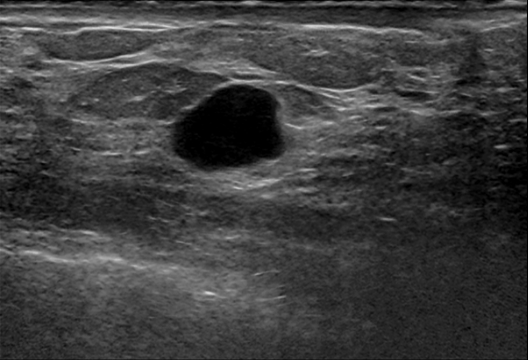
\includegraphics[width=.26\textwidth]{pngImgs/000002.png}\,
%\subfloat[]{
\begin{tikzpicture}

\node[anchor=south west,inner sep=0] (imgNode) at (0,0) {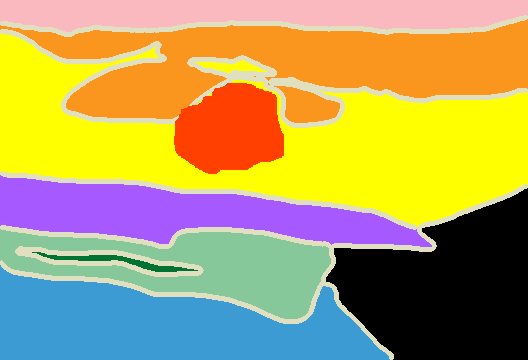
\includegraphics[width=.26\textwidth]{pngImgs/gt/000002.png}};

\node[anchor=south east,inner sep=0] at (-8pt,0) {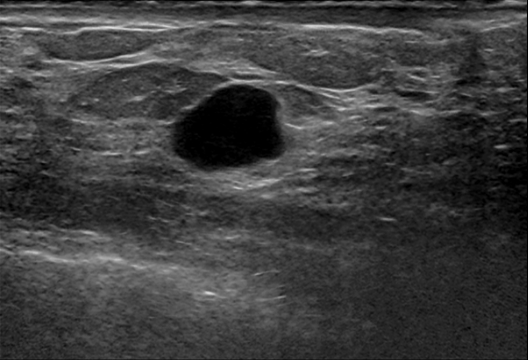
\includegraphics[width=.26\textwidth]{pngImgs/000002.png}};

\definecolor{lungColor}{rgb}{0.2353, 0.6078, 0.8235}
\definecolor{chestWallColor}{rgb}{0.5294, 0.7843, 0.6078}
\definecolor{ribColor}{rgb}{0.0000, 0.4510, 0.1961}
\definecolor{pectoralColor}{rgb}{0.6510, 0.3490, 1.0000}
\definecolor{fibroGlandColor}{rgb}{1.0000, 1.0000, 0.0000}
\definecolor{fatColor}{rgb}{0.9804, 0.5882, 0.1176}
\definecolor{skinColor}{rgb}{0.9804, 0.7255, 0.7451}
\definecolor{unkTissueColor}{rgb}{0.6000, 0.3020, 0.2510}
\definecolor{bgColor}{rgb}{0.0000, 0.0000, 0.0000}
\definecolor{lesionColor}{rgb}{1.0000, 0.2510, 0.0000}
\definecolor{boundaryColor}{rgb}{0.8784, 0.8784, 0.7529}

\tikzset{nameSt/.style=
{anchor=north west,rectangle,
node distance=5pt,
minimum width=8pt,minimum height=8pt,
}}
\begin{scriptsize}

\draw[] (imgNode.north east) +(8pt,0) node[nameSt, draw=chestWallColor, fill=chestWallColor,label=right:Chest wall] (cwName) {} ;
\draw[] node[nameSt, draw=ribColor, fill=ribColor,below=of cwName,label=right:Rib] (ribName) {} ;
\draw[] node[nameSt, draw=skinColor, fill=skinColor,below=of ribName,label=right:Skin layers] (skinName) {} ;
%\draw[] node[nameSt, draw=unkTissueColor, fill=unkTissueColor,below=of skinName,label=right:Chest wall] (unkTissueName) {} ;

\draw[] node[nameSt, draw=lesionColor, fill=lesionColor,below=of skinName,label=right:Lesion] (lesionName) {} ;
\draw[] node[nameSt, draw=boundaryColor, fill=boundaryColor,below=of lesionName,label=right:Boundary] (boundaryName) {} ;

\draw[] (imgNode.north east) +(2.2,0) node[nameSt,draw=lungColor, fill=lungColor,label=right:Air or lungs] (lungName) {};
\draw[] node[nameSt, draw=pectoralColor, fill=pectoralColor,below=of lungName,label=right:Pectoral muscle] (pectoralName) {} ;
\draw[] node[nameSt, draw=fibroGlandColor, fill=fibroGlandColor,below=of pectoralName,label=right:Fibro-glandular tissue] (fibroGlandName) {} ;
\draw[] node[nameSt, draw=fatColor, fill=fatColor,below=of fibroGlandName,label=right:Adipose tissue] (fatName) {} ;
\draw[] node[nameSt, draw=bgColor, fill=bgColor,below=of fatName,label=right:Background] (bgName) {} ;

\end{scriptsize}

%\draw[] node[nameSt,draw=Gcolor, fill=Gcolor, below=of FAname,label=right:Ganglion] (Gname) {}; 
%\draw[] node[nameSt,draw=Hcolor, fill=Hcolor, below=of Gname,label=right:Harmatoma] (Hname) {}; 
%\draw[] node[nameSt,draw=CDIcolor, fill=CDIcolor, below=of Hname,label=right:Ductal Infiltrating Carcinoma] (CDIname) {}; 
%\draw[] node[nameSt,draw=CIDcolor, fill=CIDcolor, below=of CDIname,label=right:Intra-Ductal Carcinoma] (CIDname) {}; 
%\draw[] node[nameSt,draw=CLIcolor, fill=CLIcolor, below=of CIDname,label=right:Infiltrating Lobular Carcinoma] (CLIname) {}; 
%\draw[] node[nameSt,draw=Othercolor, fill=Othercolor, below=of CLIname,label=right:Other Pathologies] (Othername) {}; 
\end{tikzpicture}
%}

\caption{Dataset sample. From left to right: image sample, accompanying multi-label \ac{gt}, tissue label \ac{gt} color-coding.}
\label{fig:dataExample}
\end{figure}

\section{Using \ac{sift} as a low-level texture descriptor in order to differentiate the tissues present in breast \acs{us} images}
%\section{Low level texture description of the breast tissue using \ac{sift} }
\acf{sift}~\cite{lowe2004distinctive} transforms key-points into scale and rotation invariant coordinates relative to local features. The \ac{sift} descriptor at a particular key-point, samples the magnitude and orientation of the gradients surrounding this key-point to generate a 128 element feature. When setting up \ac{sift} as a texture descriptor, the key-points are considered to be a regular grid in order to generate evenly sparse \ac{sift} descriptors.

%generate a texture descriptor out of \ac{sift} descriptors, a regular grid is used to generate evenly sparse \ac{sift} descriptors. At the finest resolution every single pixel of an image can be used as a key-point to extract a \ac{sift} descriptor out of every possible position.

The usage of \ac{sift} descriptor brings invariability to scale, rotation and minor affine transformations along with robustness to illumination changes~\cite{lowe2004distinctive}, which allows to characterize the tissues despite the variability from \ac{us} adquisition.

% Dense \ac{sift} uses every pixel in the image as a key-point in order to map the whole image in this space. Initially, scale and orientation of the key-points are determined. The image gradient's magnitude and orientation are then sampled according to the determined scale and orientation to generate a 128 element feature mapping each point in this hyperspace. 


Figures~\ref{fig:siftImg} to~\ref{fig:quantitativeComparison} are used to analyze both qualitatively and quantitatively the usage of \ac{sift} as a low-level descriptor to encode \ac{us} texture. In order to study the image in terms of \ac{sift} descriptors the images are mapped to this \ac{sift} space by extracting a \ac{sift} descriptor at every pixel position. In order to visually keep track of this \ac{sift}, their 128 dimensions are projected into a two dimensional space using \ac{pca}. When combining features using \ac{pca} is convenient to know the ratio known as explained variation, which is in this case is given by $\frac{\lambda_1+\lambda_2}{\sum_{i=1}^{128}\lambda_i}=21.6\%$. %This ratio, for the experiment here presented, is $21,6\%$. 
For the rest of the article all the calculation are carried out in the projected space, under the assumption that if any separability can be found, in a higher space with greater explained variation would have greater separability.
%\begin{equation}
%\frac{\lambda_1+\lambda_2}{\sum\limits_{i=1}^{128}\lambda_i}
%\label{eq:explainedVariability}
%\end{equation}
Figure~\ref{fig:siftImg} offers a visual interpretation of a breast \ac{us} image in terms of low-level \ac{sift} descriptors. On it, fig.\,\ref{fig:siftImg}a shows the scatter plot resulting from projecting all the \ac{sift} descriptors extracted from all the images within the dataset to the space described by their two principal components.
The descriptors, when projected into this two dimensional space, have 
%all the images within the dataset, at the \ac{sift} space and further project them at the space described by their two principal components. In this projected space, every sample has 
been arbitrary colored in such a manner that two close samples share similar color. In this manner, this arbitrary coloring can be used to color code the \ac{sift} descriptors and visually assess the images in terms of \ac{sift} (see fig.\,\ref{fig:siftImg}c).

\begin{figure}[Htbp]
\centering
\subfloat[]{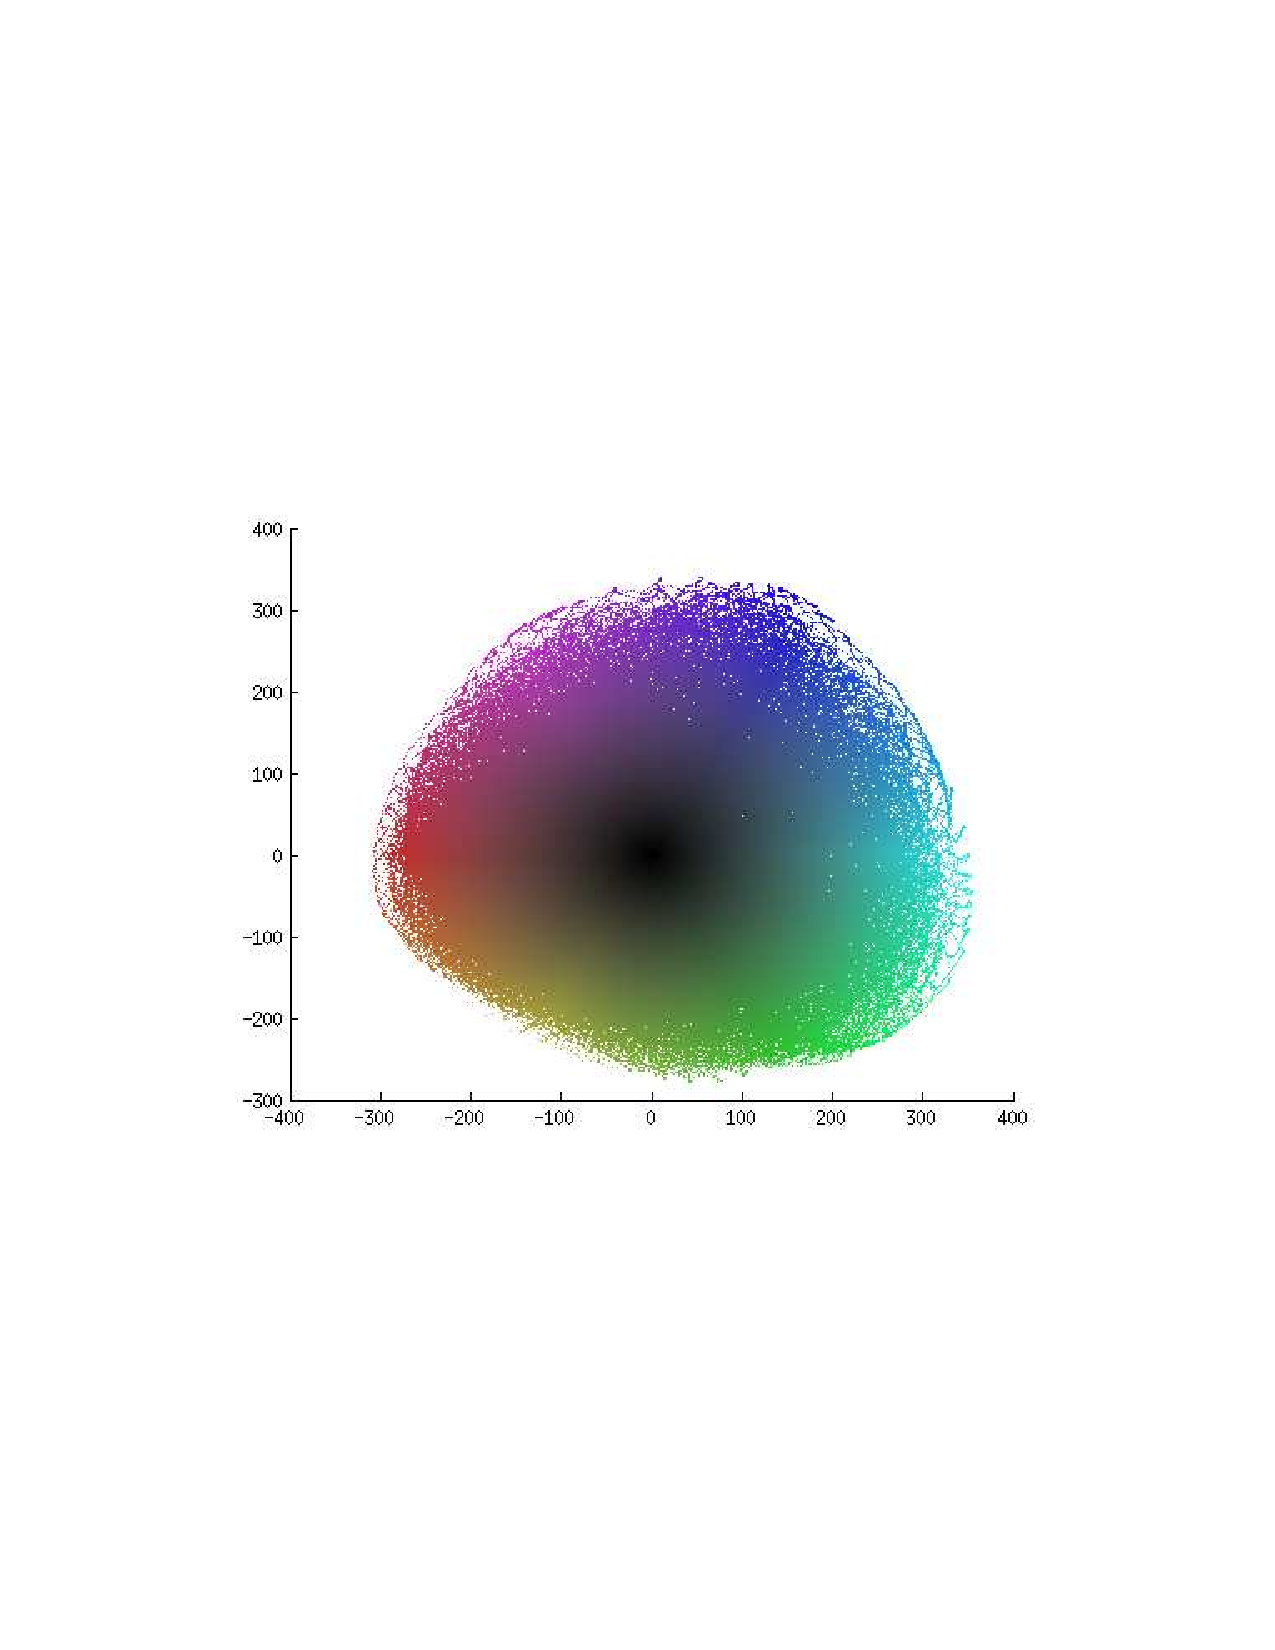
\includegraphics[trim=115 250 118 250,clip,width=.3\textwidth]{siftColorMap}}~
%\subfloat[]{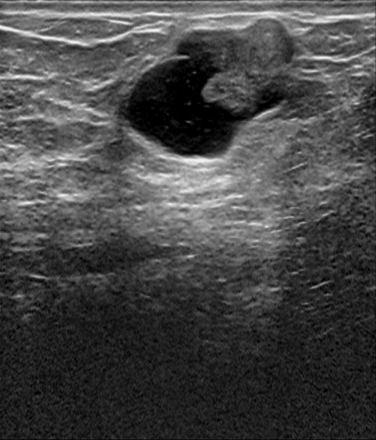
\includegraphics[height=.24\textwidth]{pngImgs/000022.png}}\,
%\subfloat[]{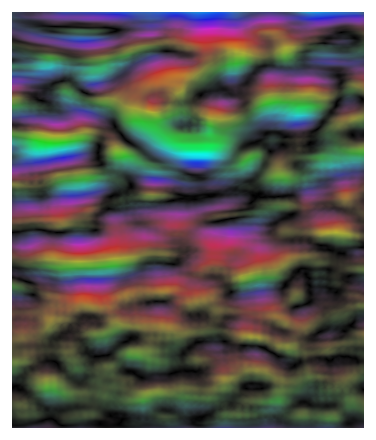
\includegraphics[height=.24\textwidth]{siftImages/000022.png}}\,
\subfloat[]{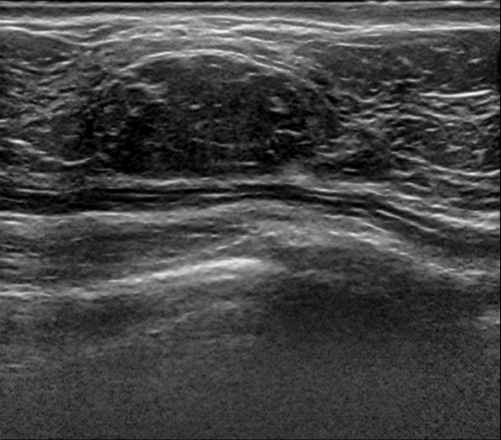
\includegraphics[height=.24\textwidth]{pngImgs/000014.png}}\,
\subfloat[]{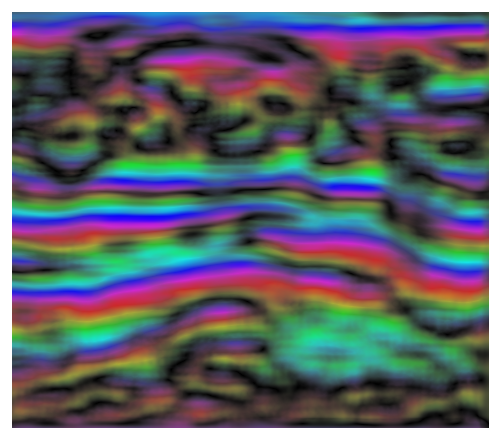
\includegraphics[height=.24\textwidth]{siftImages/000014.png}}
\caption{Low level \ac{sift} descriptor example. (a) Arbitrary coloring of the projected \acs{sift} space. (b) Original image. (c) Recoding of the extracted \ac{sift} descriptors using the color coding in (a). }
\label{fig:siftImg}
\end{figure}

In order to analyze the tissue distribution in this texture space of \ac{sift} descriptors, the analysis of the \ac{map} estimator has been chosen, as described in equation~\ref{eq:bayes}.% The model is presented in equation~\ref{eq:bayes} and figures~\ref{fig:siftMapping} to~\ref{fig:sift_and_ingensity_MAP} visually interprets its terms.

\begin{equation}
P(\omega|\bar{x}_a) = \frac{P(\bar{x}_a|\omega)\cdot P(\omega)}{P(\bar{x}_a)}
\label{eq:bayes}
\end{equation}

Where $P(\omega|\bar{x}_a)$ is the probability that the sample $a$ belongs to class $\omega \in W$ (see fig.\,\ref{fig:dataExample}b as a reminder of the \ac{gt} available classes) based on $\bar{x}_a$ which is the feature vector representing the sample $a$, such that $x_a^i$ is the $i$th feature. $P(\bar{x}_a|\omega)$ corresponds to the \ac{ml} of the feature distribution for a particular class $\omega$, while $P(\omega)$ and $P(\bar{x}_a)$ are the priors for the class and feature respectively.

Figure~\ref{fig:siftMapping} \todo{alin the figures in fig. \ref{fig:siftMapping}} uses the entire dataset to illustrate the underlying problem and the priors extracted from the same dataset. Fig.\,\ref{fig:siftMapping}a shows a scatter plot where every sample has been colored according to its \ac{gt}. Fig.\,\ref{fig:siftMapping}b shows an occurrence study of the samples carried out in a discretization of the space in fig.\,\ref{fig:siftMapping}a that illustrates the distribution of the \ac{sift} descriptors present within the images, which corresponds to the $P(\bar{x}_a)$ term in eq.\,\ref{eq:bayes}. Fig.\,\ref{fig:siftMapping}c illustrates the class prior corresponding to the proportion of samples present in the dataset for each class.

\begin{figure}[Htbp]
\centering
%\subfloat[]{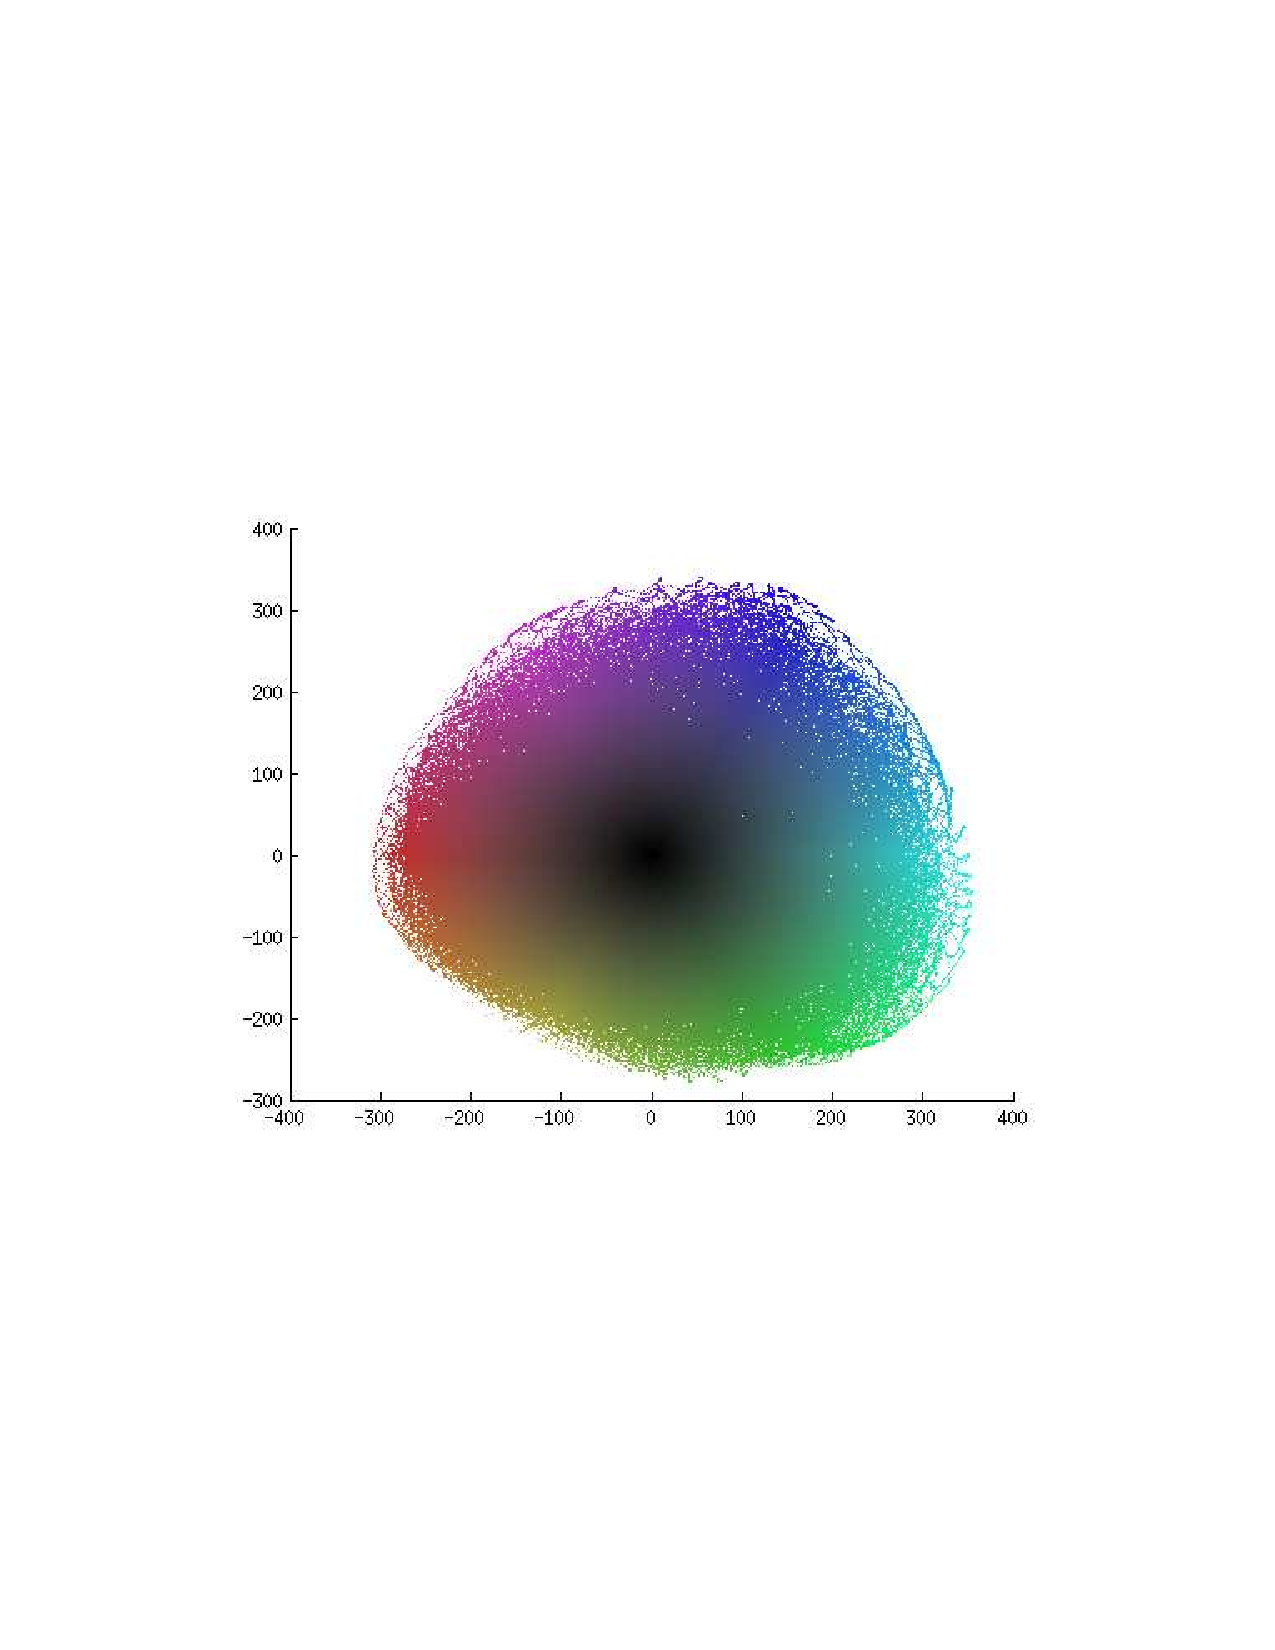
\includegraphics[trim=115 250 118 250,clip,width=.3\textwidth]{siftColorMap}}\,
%\subfloat[]{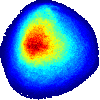
\includegraphics[width=.24\textwidth,angle = 90]{siftOccurrences}}\,
\subfloat[]{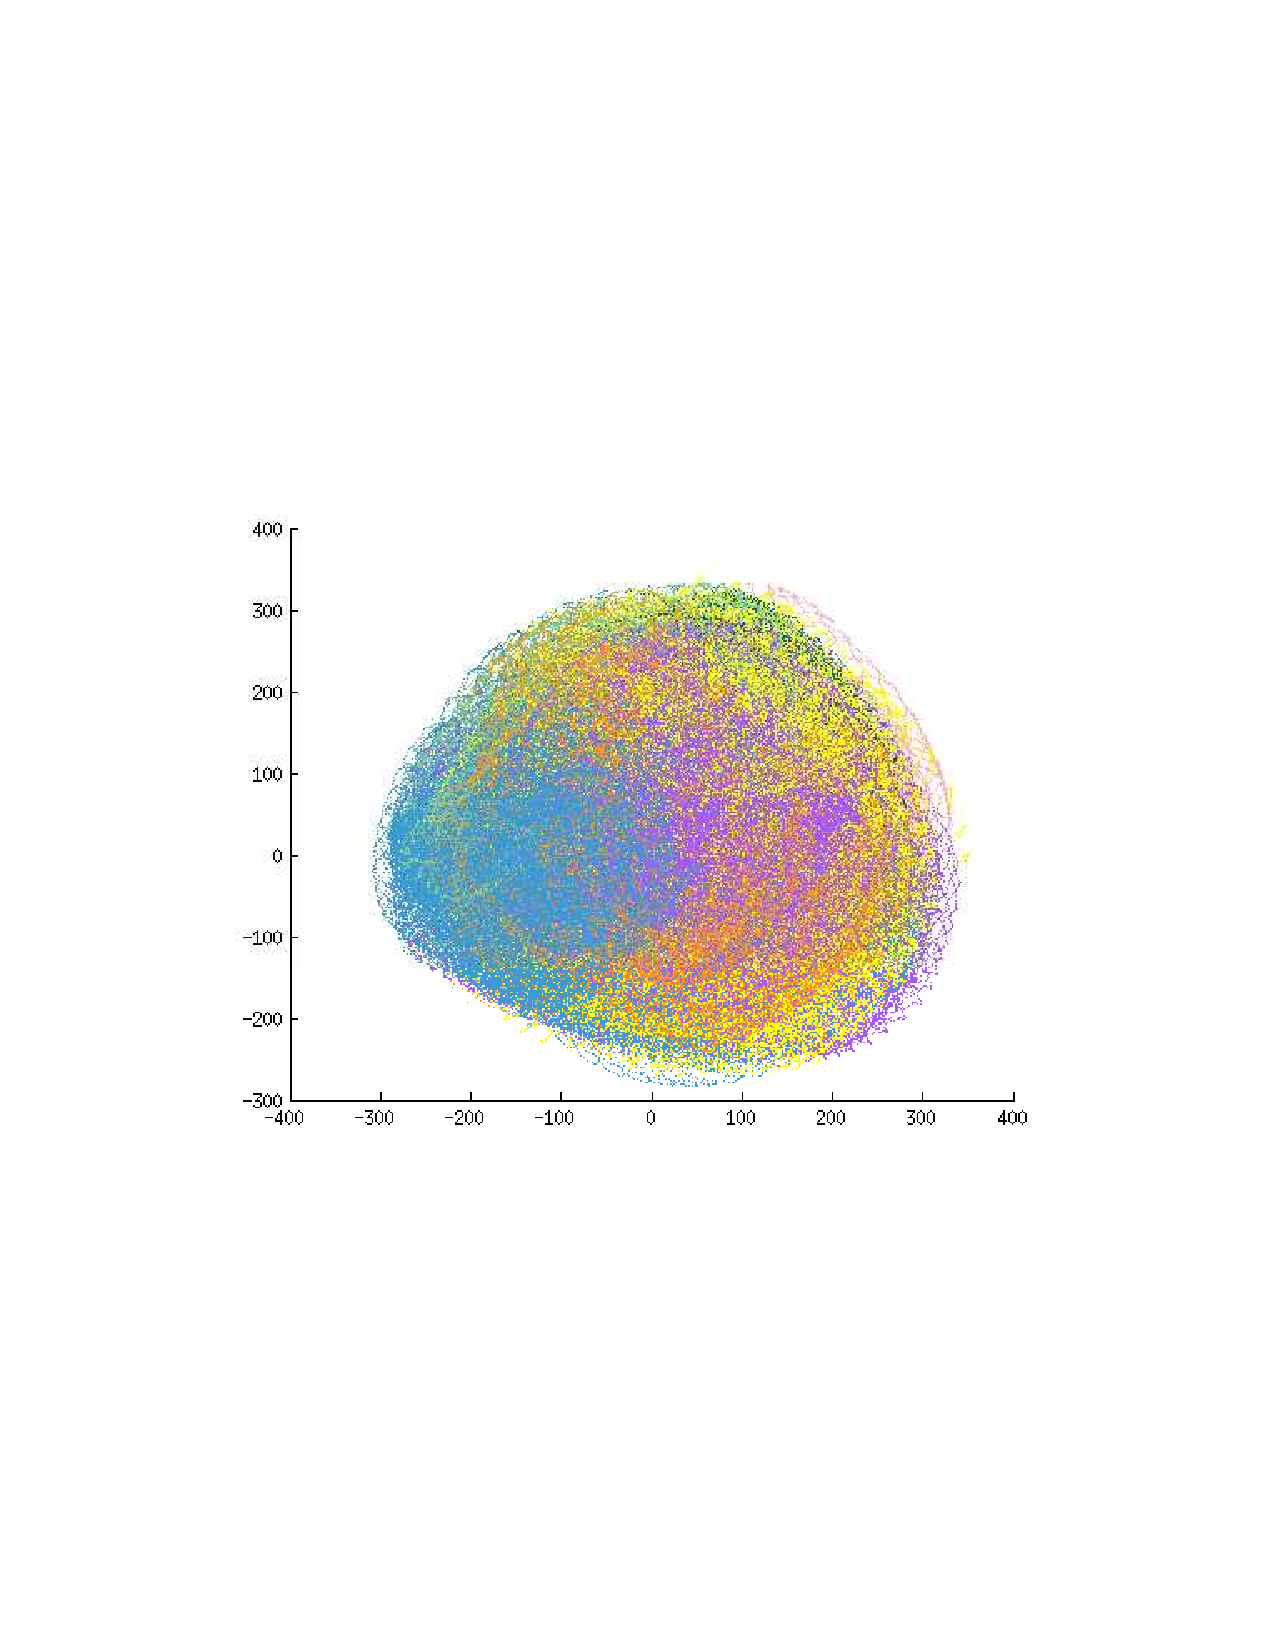
\includegraphics[trim=115 250 118 250,clip,width=.3\textwidth]{mapGTintoSIFT}}\quad
\subfloat[]{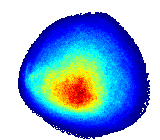
\includegraphics[width=.24\textwidth,]{siftOccurrences2}}
\subfloat[]{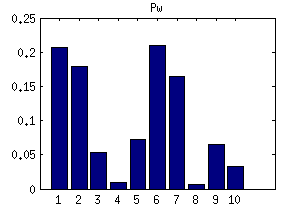
\includegraphics[width=.24\textwidth,]{classPrior}}

%\caption{2D visualization of the \acs{sift} hyper space. (a) Arbitrary color coding of the projected space. (b) Occurrence density. (c) Projected space colored according to \acs{gt} tissue labeling.}
\caption{2D visualization of the \acs{sift} hyper space. (a) Projected space colored according to \acs{gt} tissue labeling. (b) Occurrence density.}
\label{fig:siftMapping}
\end{figure}



Figure~\ref{fig:P_class_knowing_features} shows the feature distribution study for every class, corresponding to the $P(\bar{x}_a|\omega)$ in eq.\,\ref{eq:bayes}. On it, tendencies of features for representing different classes can be observed illustrating the similarities and dissimilarities between classes. As example the reader is referred to fig.~\ref{fig:dataExample} to illustrate the fact that adipose tissue class contains Cooper's ligaments which are highly dense fibers, and fibro-glandular tissue is made of dense fibers and unstructured fat. Or, the difficulty of producing accurate \ac{gt} delineations. Take for instance the label background which is meant for regions where the breast structures are no clear enough for the reader. A concept which is highly reader dependent.

\begin{figure}[Htbp]
\centering
 \begin{tikzpicture}

\tikzset{myNode/.style=
{anchor=north west,rectangle,
node distance=5pt,
minimum width=8pt,minimum height=8pt,
inner sep=0,
}}

\node[myNode, label=below:Background] (bgNode) at (0,0) {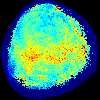
\includegraphics[width=.25\textwidth]{gtDistro/000.png}};
\node[myNode, right=of bgNode, label=below:Air or lungs] (airNode) {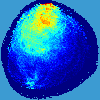
\includegraphics[width=.25\textwidth]{gtDistro/001.png}};
\node[myNode, right=of airNode, label=below:Chest wall] (cwNode) {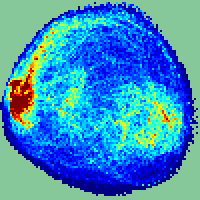
\includegraphics[width=.25\textwidth]{gtDistro/002.png}};

\node[myNode, right=of cwNode, label=below:Rib] (ribNode) {
\includegraphics[width=.25\textwidth]{gtDistro/003.png}};
%\node[myNode, right=of ribNode, label=below:Pectoral muscle] (pecNode) {
\includegraphics[width=.25\textwidth]{gtDistro/004.png}};

\node[myNode, below=15pt of bgNode, label=below:Fibro-glandular] (fibNode) {
\includegraphics[width=.25\textwidth]{gtDistro/005.png}};

\node[myNode, right=of fibNode, label=below:Adipose tissue] (fatNode) {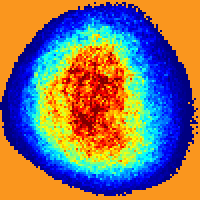
\includegraphics[width=.25\textwidth]{gtDistro/006.png}};
\node[myNode, right=of fatNode, label=below:Skin layers] (skNode) {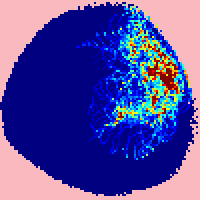
\includegraphics[width=.25\textwidth]{gtDistro/007.png}};
\node[myNode, right=of skNode, label=below:Lesion] (lesionNode) {
\includegraphics[width=.25\textwidth]{gtDistro/128.png}};

%\node[myNode, label=below:Background] (bgNode) at (0,0) {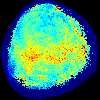
\includegraphics[width=.25\textwidth]{gtDistro/000.png}};
%\node[myNode, right=of bgNode, label=below:Air or lungs] (airNode) {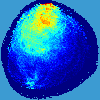
\includegraphics[width=.25\textwidth]{gtDistro/001.png}};
%\node[myNode, right=of airNode, label=below:Chest wall] (cwNode) {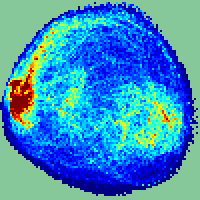
\includegraphics[width=.25\textwidth]{gtDistro/002.png}};
%
%\node[myNode, below=15pt of bgNode, label=below:Rib] (ribNode) {
\includegraphics[width=.25\textwidth]{gtDistro/003.png}};
%\node[myNode, right=of ribNode, label=below:Pectoral muscle] (pecNode) {
\includegraphics[width=.25\textwidth]{gtDistro/004.png}};
%\node[myNode, right=of pecNode, label=below:Fibro-glandular] (fibNode) {
\includegraphics[width=.25\textwidth]{gtDistro/005.png}};
%
%\node[myNode, below=15pt of ribNode, label=below:Adipose tissue] (fatNode) {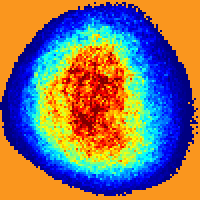
\includegraphics[width=.25\textwidth]{gtDistro/006.png}};
%\node[myNode, right=of fatNode, label=below:Skin layers] (skNode) {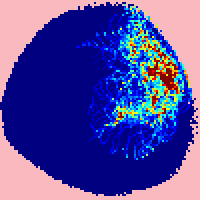
\includegraphics[width=.25\textwidth]{gtDistro/007.png}};
%\node[myNode, right=of skNode, label=below:Lesion] (lesionNode) {
\includegraphics[width=.25\textwidth]{gtDistro/128.png}};


\end{tikzpicture} \\
\caption{Distribution of the \acs{sift} descriptors for some classes in the \ac{gt}}%tissues present in breast \ac{us} images.}%. The background color codes the tissue type.}
\label{fig:P_class_knowing_features}
\end{figure}

Using eq.\,\ref{eq:bayes} a \ac{map} estimation of the probability for each class can be calculated at every position based on the data shown in fig.\,\ref{fig:siftMapping} and fig.\,\ref{fig:P_class_knowing_features}.
Equation~\ref{eq:labeling} illustrates produce the preferred labeling of the space which is illustrated in figure~\ref{fig:sift_and_ingensity_MAP}a. On it, the marginals $P(\omega_i|x^j)$ where $j\in \{1,2\}$ are also represented to obtain a deeper understanding of the \ac{map}.

\begin{equation}
labeling(\bar{x}) = \quad\underset{i}{\arg\max}\quad P(\omega_i|\bar{x})
\label{eq:labeling} \qquad \text{where } i \in [1 .. |W|] 
\end{equation}

For comparison purposes, figure~\ref{fig:sift_and_ingensity_MAP} is complemented by repeating the experiment carried out in fig.figure~\ref{fig:sift_and_ingensity_MAP}a, this time using intensity as single feature such that $x_a \in [0 .. 255]$ (see fig.~\ref{fig:sift_and_ingensity_MAP}b). When comparing both labeled spaces, the \ac{sift} feature is preferred since exist no mode for some of the classes when using intensity.

% Figure~\ref{fig:mapQualitativeResults}a colors the space based on the most probable class. As it can be observed, the coloring of the space is mostly congruent indicating that each tissue is grouped within the \ac{sift} which facilitates class separability. This coloring of the space can be used as a Bayesian classification of the sample. Figure~\ref{fig:mapQualitativeResults}c \todo{falta la imatge}  shows the result of this classification from an unseen image (see fig.\,\ref{fig:mapQualitativeResults}b). Since no multi-label \ac{gt} is present for this image only qualitative assessment of the results can be made. 
%\todo[inline]{In order to improve the results, MRF can be used to ensure spatial coherence for the labeling. Also instead of only using the map, the reward obtained from the other classes can also be taken into account. similar classes are easily mislabeled ej: background and lungs, fibro-glandular and fat}

%\begin{figure}[Htbp]
%\centering
%\subfloat[]{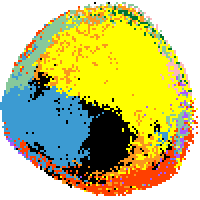
\includegraphics[width=.24\textwidth]{gtDistro/mapLabeling.png}}\,
%\subfloat[]{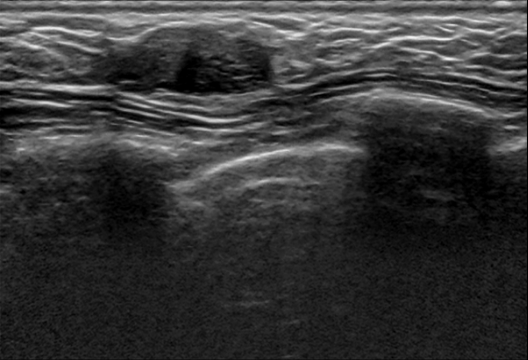
\includegraphics[width=.265\textwidth]{pngImgs/000011.png}}\,
%\subfloat[]{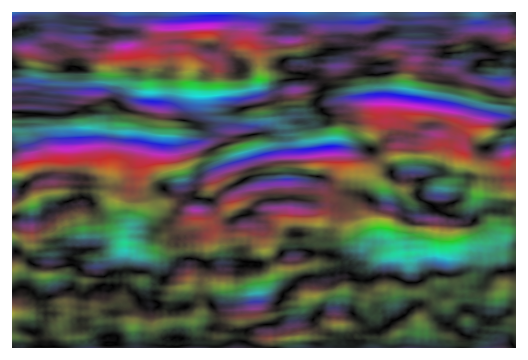
\includegraphics[width=.265\textwidth]{/home/sik/Work/escola/recerca/iwdm2014/code/gtPredictedLabel/000011.png}}
%\caption{ Qualitative results. (a) \ac{map} class label distribution of the 2D projection of the \ac{sift} descriptors. (b) unseen image (c) image labeling results}
%\label{fig:mapQualitativeResults}
%\end{figure}

\begin{figure}[Htbp]
\centering
\subfloat[SIFT]{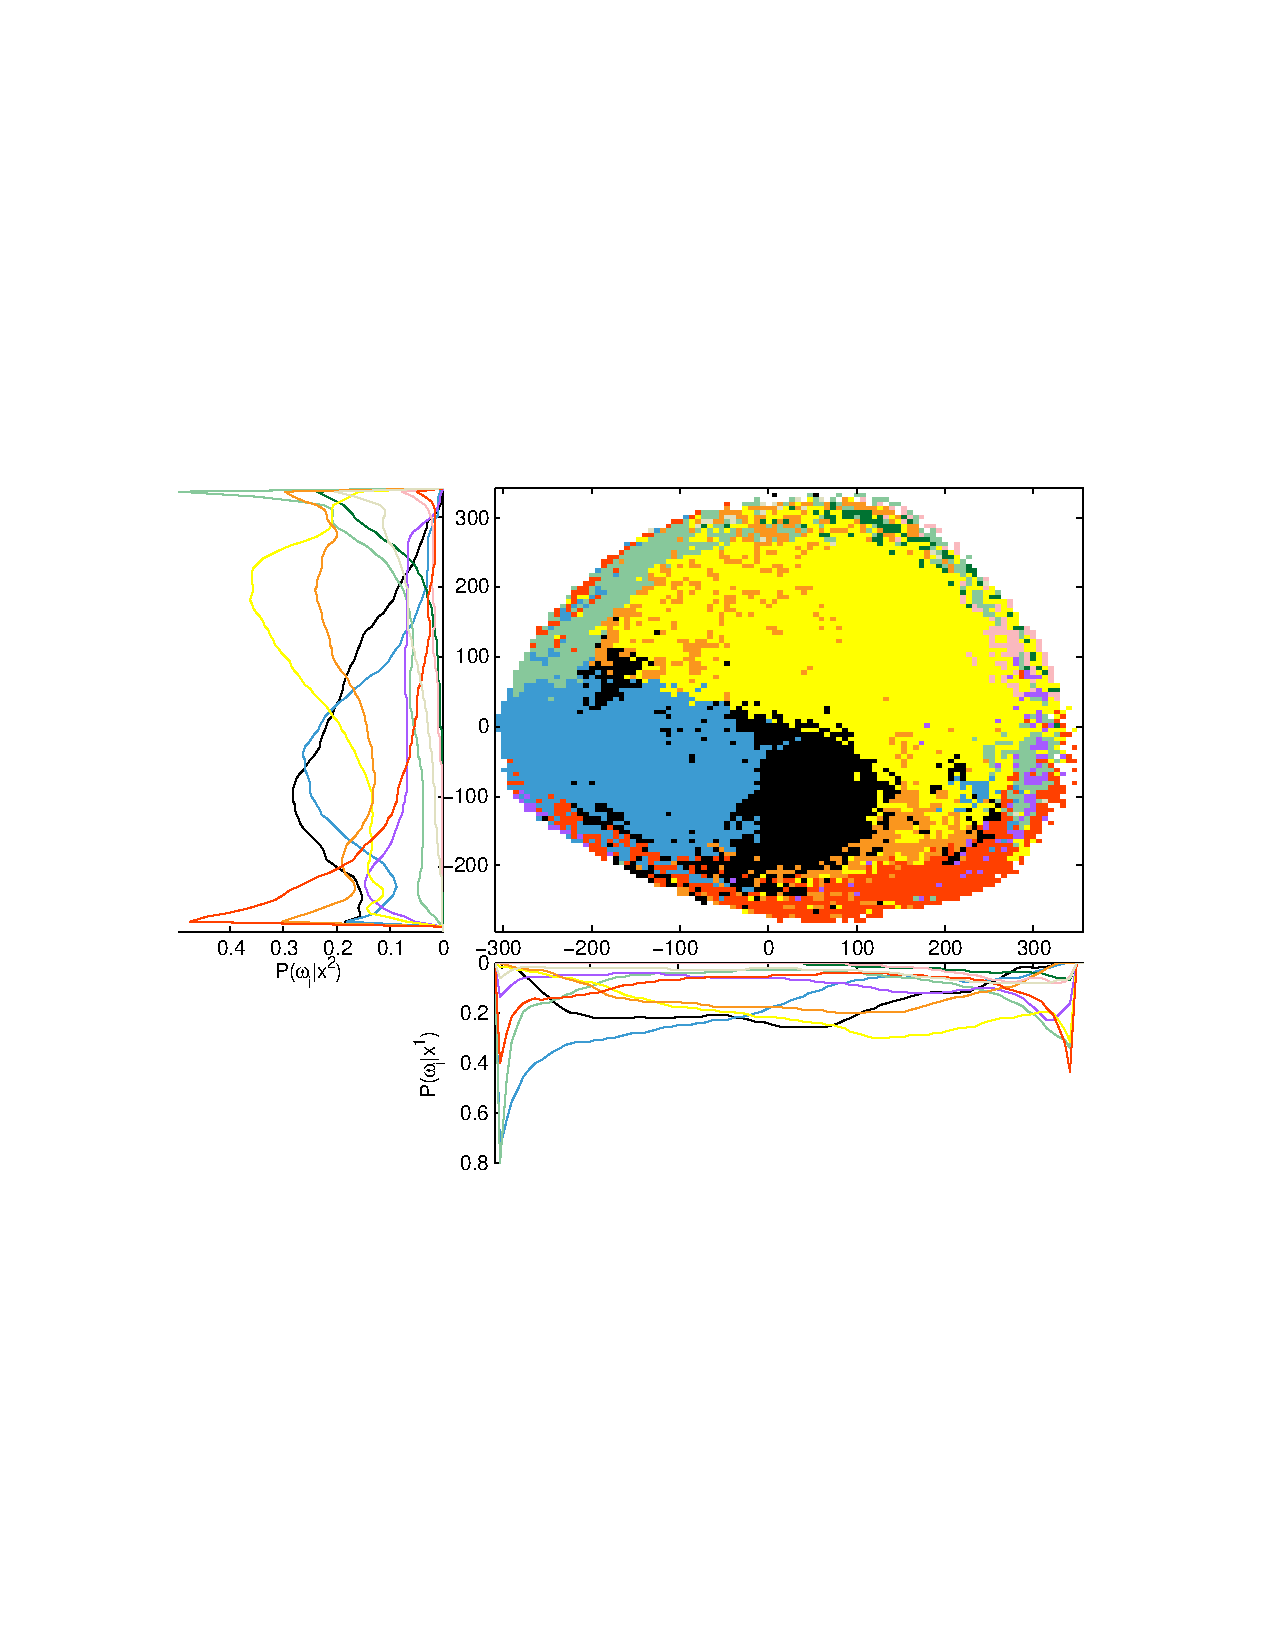
\includegraphics[trim = 91 230 90 230, clip,width=.5\textwidth]{labelingMAP.pdf}}\quad
\subfloat[Intensity]{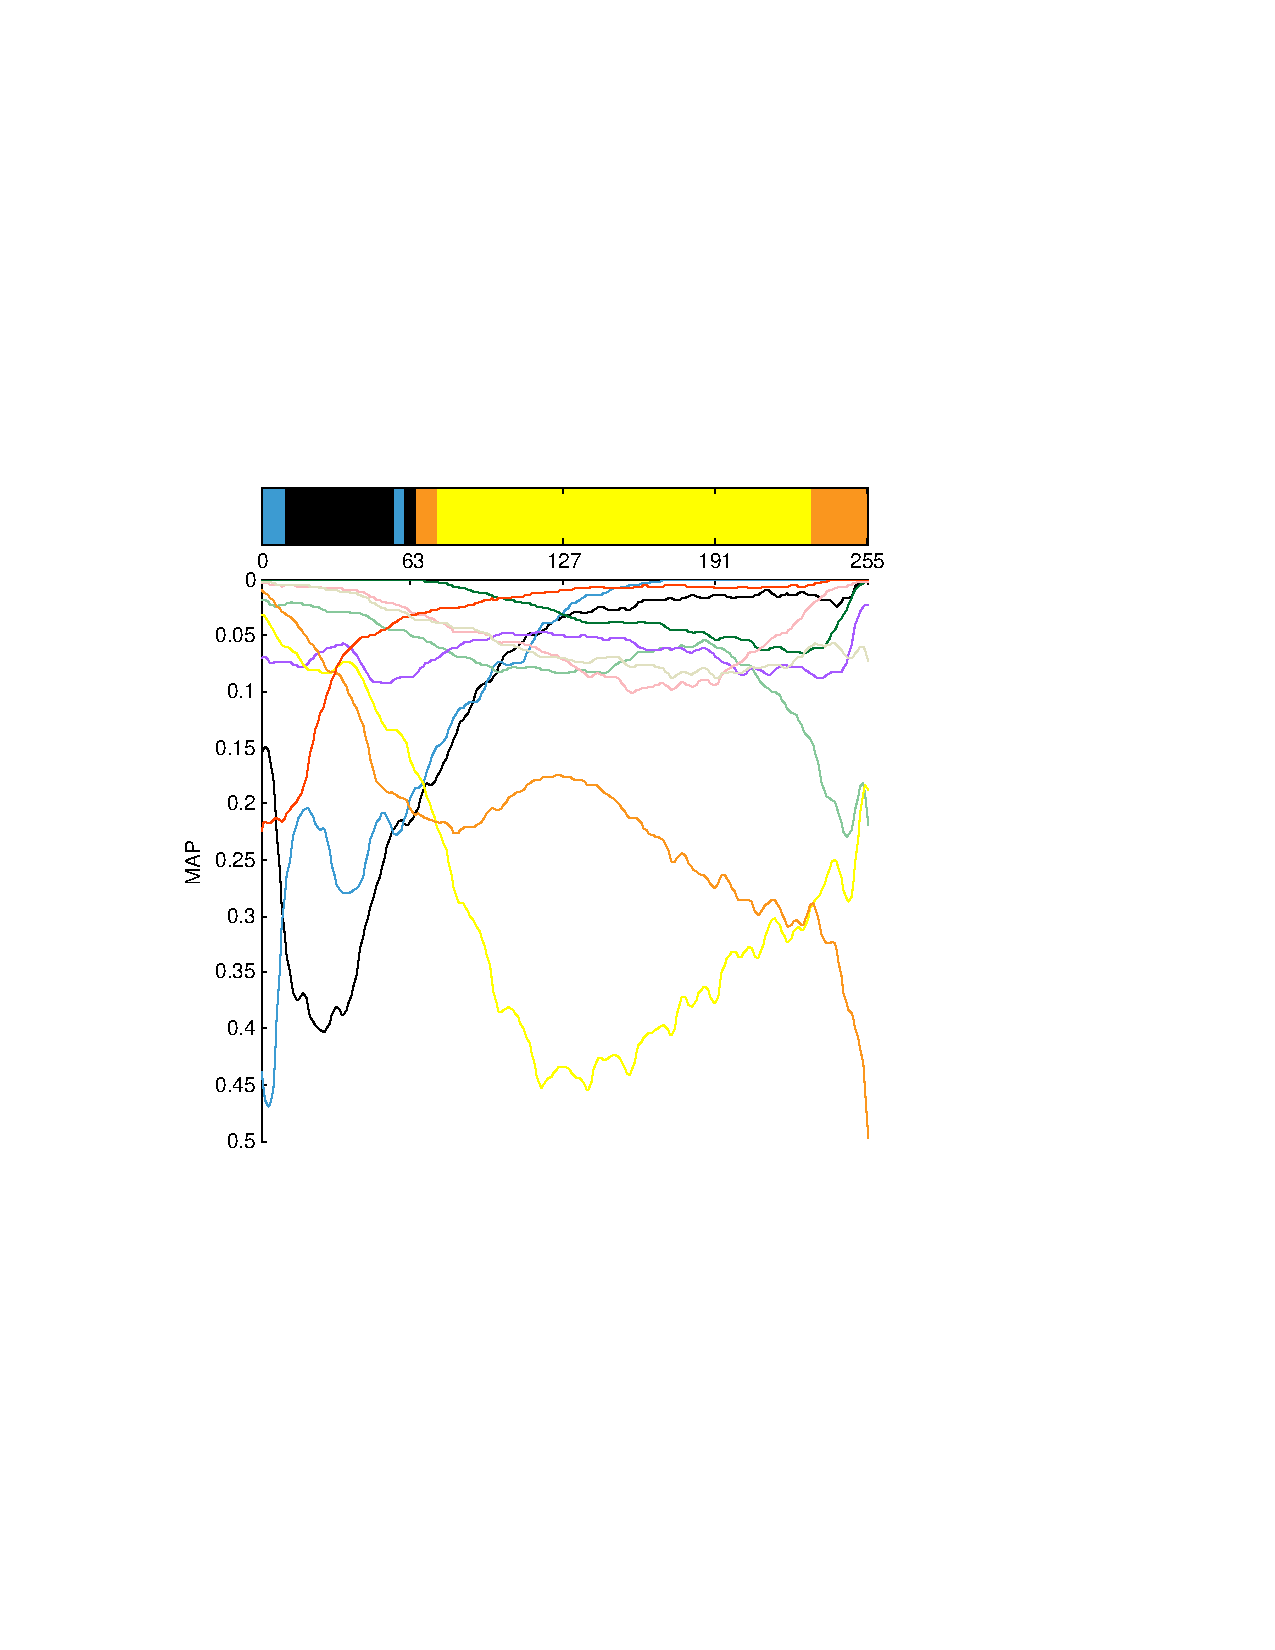
\includegraphics[trim = 85 230 180 230, clip,width=.4\textwidth]{intensityLabelingMAP.pdf}}\\
%\subfloat[]{\includegraphics[trim = 91 250 100 242, clip,width=.4\textwidth]{/home/sik/Work/escola/recerca/iwdm2014/code/sift1map.pdf}}\,
%\subfloat[]{\includegraphics[trim = 91 250 100 242, clip,width=.4\textwidth]{/home/sik/Work/escola/recerca/iwdm2014/code/sift2map.pdf}}
\caption{ Qualitative evaluation of the \ac{map} labeling of the feature space .}
\label{fig:sift_and_ingensity_MAP}
\end{figure}

%\subsection{Quantitative assessing}
In order to generate cross-validated quantitative results, it has been sampled from the dataset, 5 folds of 10.000 samples for each class per fold. At each round 4 folds have been used for training the \ac{ml} term in eq.\,\ref{eq:bayes} ($P(\bar{x}_a|\omega)$) and the ramaining fold has been used for testing the classification. Figure~\ref{fig:quantitativeComparison} uses boxplots to illustrate the distribution of the confusion matrix across the folds. In the figure, the samples are grouped by the actual class of the sample and divided by the predicted classes. The top label represents the samples' actual class, whereas the predicted class is color coded at the bottom. Boxplots in blue represent the results of classifying the samples using intensity, whereas the bloxpots in red represent the results obtained when using \ac{sift}. The lack of variability within the boxplots illustrates a repeatability of the results across the samples, which gets accentuated when using \ac{sift}. The results show that the preferred labels which cover larger portion of the feature space achieve better results than the other classes. This is more clear for the intensity case since there are classes with no mode and therefore all the samples of this class are misclassified (see fig.~\ref{fig:sift_and_ingensity_MAP}). The sensitivity or \ac{tpr} allows to obtain a general sense of performance across all the labels. The \ac{tpr} value obtained for the intensity case is $16.6\pm27.5\%$, whereas for the \ac{sift} case is $18.8\pm17.2\%$ which show that both feature spaces produce similar results. Notice that the large variability reported is due to missclassification of the labels with no mode, as can be observed in figure~\ref{fig:sift_and_ingensity_MAP}.

%\begin{figure}[Htbp]
%\centering
%\subfloat[]{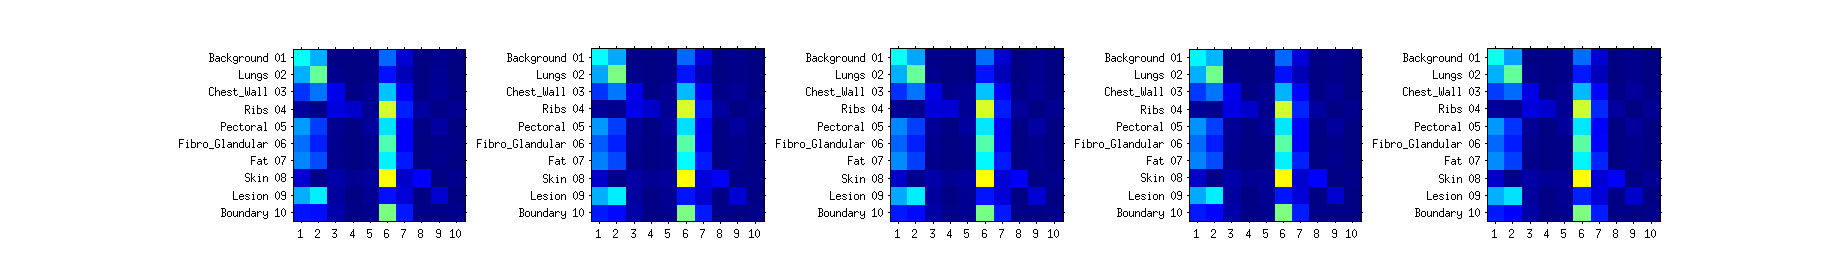
\includegraphics[width=\textwidth]{untitled}}
%\caption{}
%\label{fig:mapQuantitativeResults}
%\end{figure}


\begin{figure}[Htbp]
\documentclass{standalone}
\usepackage{tikz} 
\usepackage{epsf,graphicx,subfig}
\usepackage{color}
\usepackage{amssymb,amsmath}
\usepackage{scalefnt}
\usetikzlibrary{positioning}
%include other needed packages here   
\begin{document}

\begin{tikzpicture}

\definecolor{lungColor}{rgb}{0.2353, 0.6078, 0.8235}
\definecolor{chestWallColor}{rgb}{0.5294, 0.7843, 0.6078}
\definecolor{ribColor}{rgb}{0.0000, 0.4510, 0.1961}
\definecolor{pectoralColor}{rgb}{0.6510, 0.3490, 1.0000}
\definecolor{fibroGlandColor}{rgb}{1.0000, 1.0000, 0.0000}
\definecolor{fatColor}{rgb}{0.9804, 0.5882, 0.1176}
\definecolor{skinColor}{rgb}{0.9804, 0.7255, 0.7451}
\definecolor{unkTissueColor}{rgb}{0.6000, 0.3020, 0.2510}
\definecolor{bgColor}{rgb}{0.0000, 0.0000, 0.0000}
\definecolor{lesionColor}{rgb}{1.0000, 0.2510, 0.0000}
\definecolor{boundaryColor}{rgb}{0.8784, 0.8784, 0.7529}


\tikzset{nameSt/.style=
{anchor=north west,rectangle,
node distance=60.7pt,
minimum width=5pt,minimum height=5pt,
}}



\node[anchor=south west,inner sep=0] (imgNode) at (0,0) {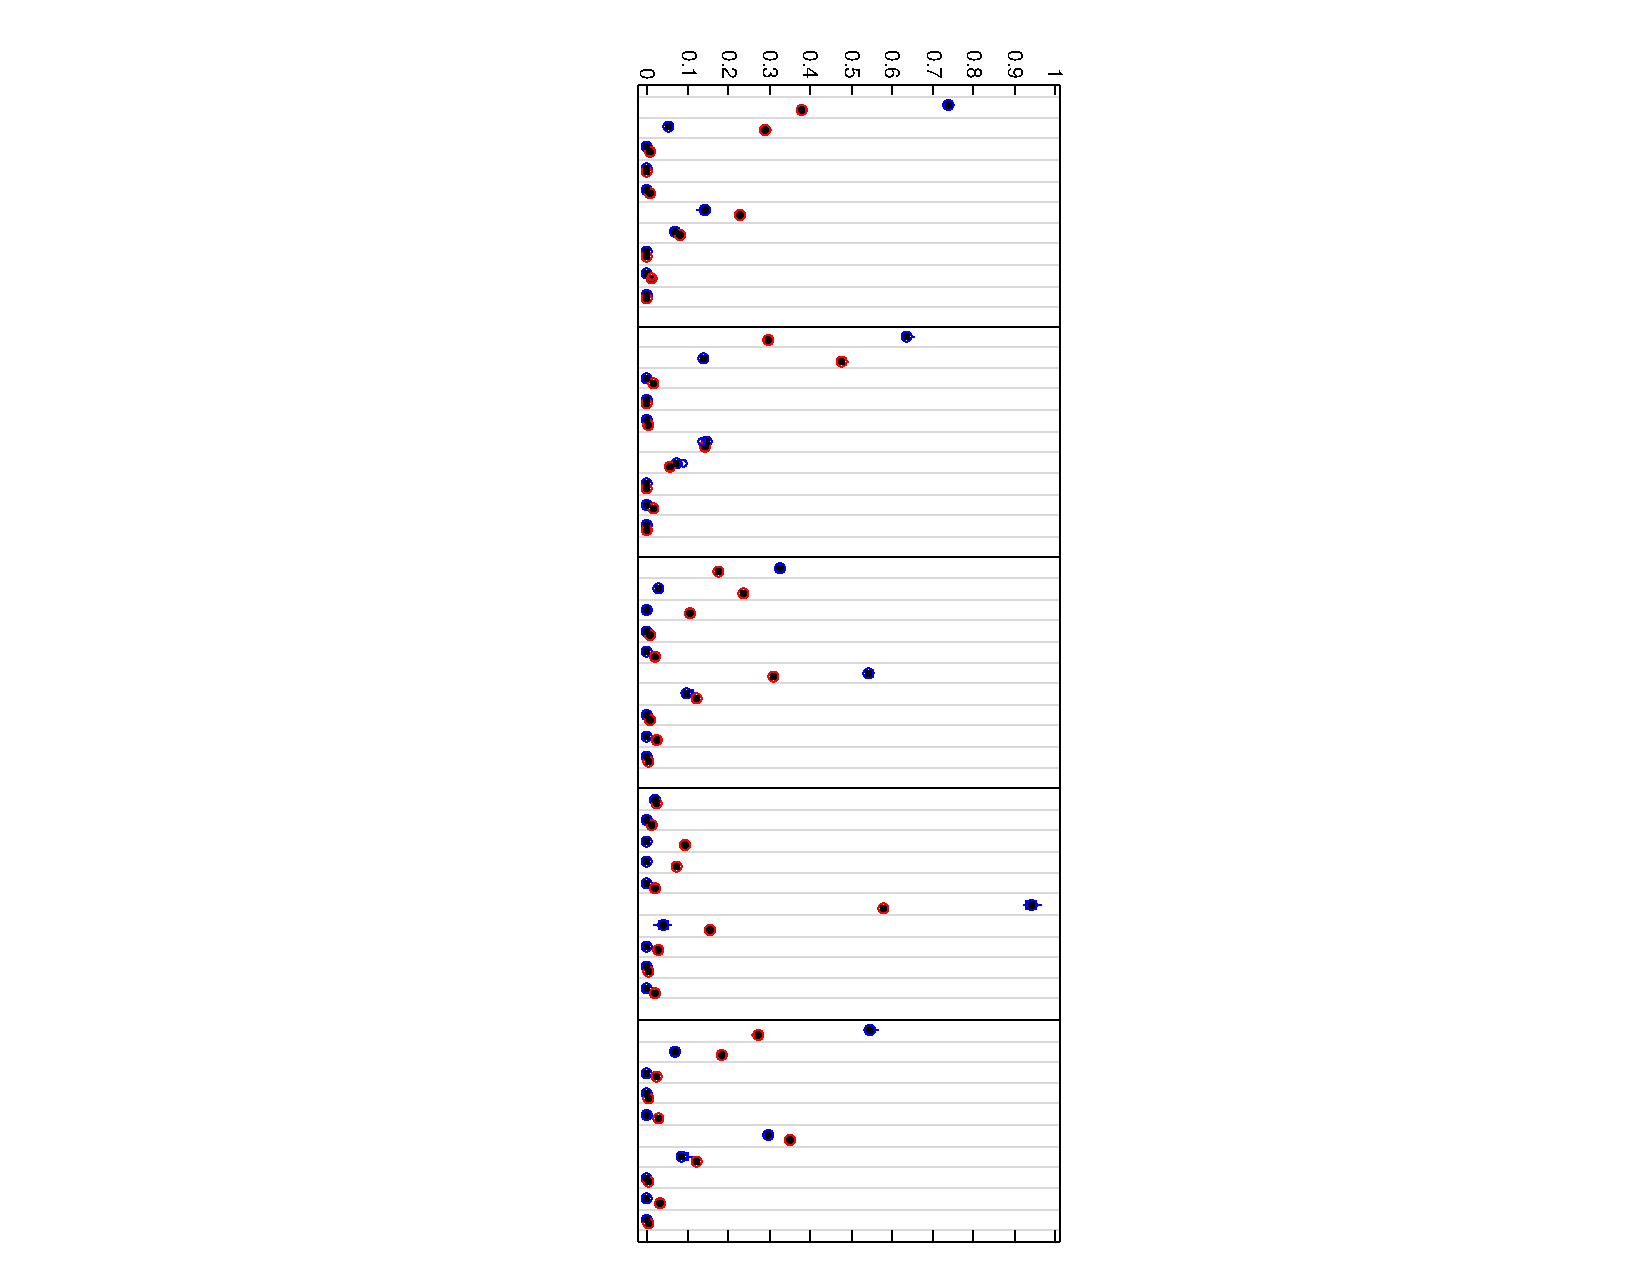
\includegraphics[trim = 305 14 277 20, clip,angle=90,width=\textwidth]{cooccurrenceMatrixA.pdf}};

\begin{tiny}

\draw[] (imgNode.north west) +(18pt,4pt) node[nameSt, draw=bgColor, fill=bgColor,label=right:Background] (bgName) {} ;
\draw[] (imgNode.north east) +(2.2,0) node[nameSt,draw=lungColor, fill=lungColor,right=of bgName,label=right:Air or lungs] (lungName) {};
\draw[] (0,0) node[nameSt, draw=chestWallColor,right=of lungName, fill=chestWallColor,label=right:Chest wall] (cwName) {} ;
\draw[] node[nameSt, draw=ribColor, fill=ribColor,right=of cwName,label=right:Rib] (ribName) {} ;
\draw[] node[nameSt, draw=pectoralColor, fill=pectoralColor,right=of ribName,label=right:Pectoral muscle] (pectoralName) {} ;

\tikzset{labelSt/.style=
{anchor=north west,rectangle,
node distance=2.6pt,
scale=.7,
minimum width=1pt,minimum height=1pt,
}}


\draw[] (imgNode.south west) +(17pt,0) node[labelSt, draw=bgColor, fill=bgColor] (bgName) {} ;
\draw[] node[labelSt,draw=lungColor, fill=lungColor,right=of bgName] (lungName) {};
\draw[] node[labelSt, draw=chestWallColor,right=of lungName, fill=chestWallColor] (cwName) {} ;
\draw[] node[labelSt, draw=ribColor, fill=ribColor,right=of cwName] (ribName) {} ;
\draw[] node[labelSt, draw=pectoralColor, fill=pectoralColor,right=of ribName] (pectoralName) {} ;
\draw[] node[labelSt, draw=fibroGlandColor, fill=fibroGlandColor,right=of pectoralName] (fibroGlandName) {} ;
\draw[] node[labelSt, draw=fatColor, fill=fatColor,right=of fibroGlandName] (fatName) {} ;
\draw[] node[labelSt, draw=skinColor, fill=skinColor,right=of fatName] (skinName) {} ;
\draw[] node[labelSt, draw=lesionColor, fill=lesionColor,right=of skinName] (lesionName) {} ;
\draw[] node[labelSt, draw=boundaryColor, fill=boundaryColor,right=of lesionName] (boundaryName) {} ;


\draw[] (imgNode.south west) +(17pt,-5) node[labelSt, draw=bgColor, fill=bgColor] (bgName) {} ;
\draw[] node[labelSt,draw=lungColor, fill=lungColor,right=of bgName] (lungName) {};
\draw[] node[labelSt, draw=chestWallColor,right=of lungName, fill=chestWallColor] (cwName) {} ;
\draw[] node[labelSt, draw=ribColor, fill=ribColor,right=of cwName] (ribName) {} ;
\draw[] node[labelSt, draw=pectoralColor, fill=pectoralColor,right=of ribName] (pectoralName) {} ;
\draw[] node[labelSt, draw=fibroGlandColor, fill=fibroGlandColor,right=of pectoralName] (fibroGlandName) {} ;
\draw[] node[labelSt, draw=fatColor, fill=fatColor,right=of fibroGlandName] (fatName) {} ;
\draw[] node[labelSt, draw=skinColor, fill=skinColor,right=of fatName] (skinName) {} ;
\draw[] node[labelSt, draw=lesionColor, fill=lesionColor,right=of skinName] (lesionName) {} ;
\draw[] node[labelSt, draw=boundaryColor, fill=boundaryColor,right=of lesionName] (boundaryName) {} ;

\node[anchor=south west,inner sep=0] (imgNode) at (0,-5) {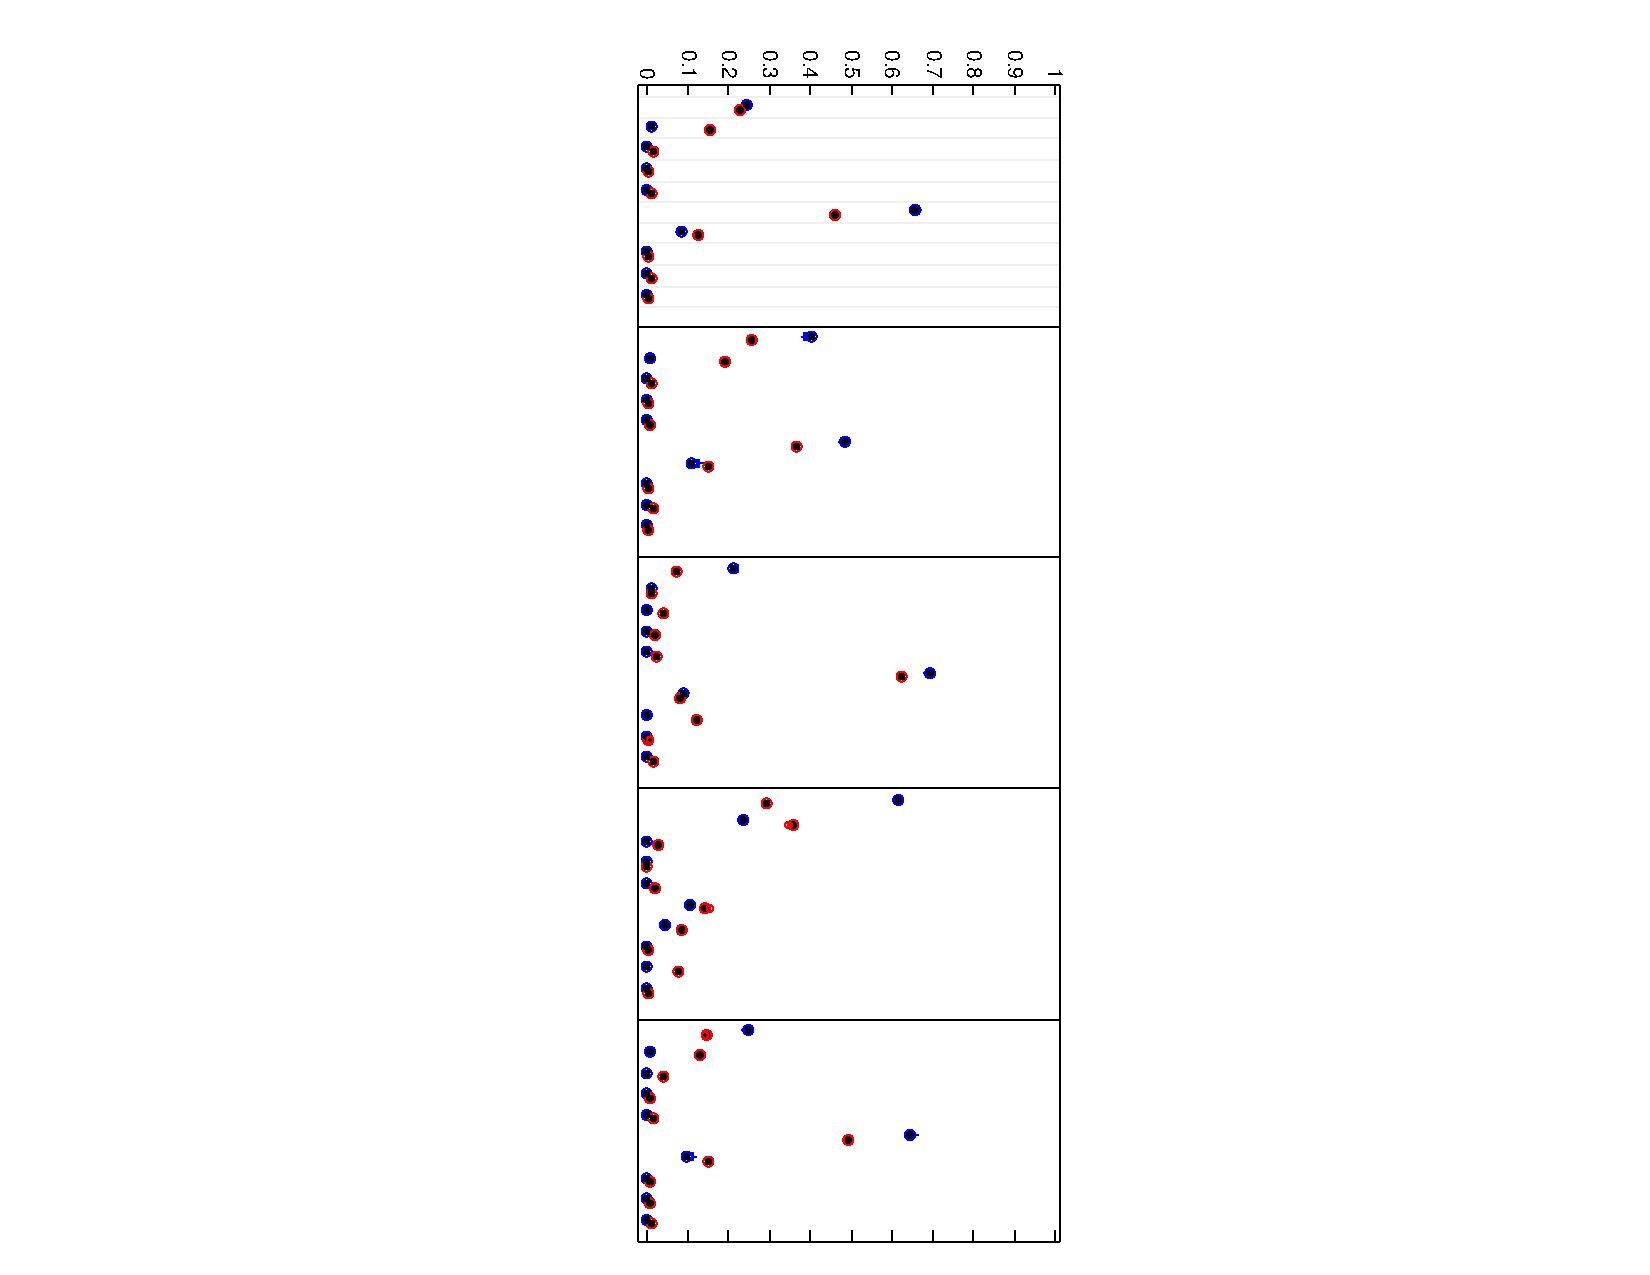
\includegraphics[trim = 305 14 277 20, clip,angle=90,width=\textwidth]{cooccurrenceMatrixB.pdf}};

\draw[] (imgNode.north west) +(18pt,4pt) node[nameSt, draw=fibroGlandColor, fill=fibroGlandColor,label=right:Fibro-glandular] (fibroGlandName) {} ;
\draw[] node[nameSt, draw=fatColor, fill=fatColor,right=of fibroGlandName,label=right:Adipose tissue] (fatName) {} ;
\draw[] node[nameSt, draw=skinColor, fill=skinColor,right=of fatName,label=right:Skin layers] (skinName) {} ;
\draw[] node[nameSt, draw=lesionColor, fill=lesionColor,right=of skinName,label=right:lesion] (lesionName) {} ;
\draw[] node[nameSt, draw=boundaryColor, fill=boundaryColor,right=of lesionName,label=right:Boundary] (boundaryName) {} ;

\end{tiny}




%\draw[] node[nameSt,draw=Gcolor, fill=Gcolor, below=of FAname,label=right:Ganglion] (Gname) {}; 
%\draw[] node[nameSt,draw=Hcolor, fill=Hcolor, below=of Gname,label=right:Harmatoma] (Hname) {}; 
%\draw[] node[nameSt,draw=CDIcolor, fill=CDIcolor, below=of Hname,label=right:Ductal Infiltrating Carcinoma] (CDIname) {}; 
%\draw[] node[nameSt,draw=CIDcolor, fill=CIDcolor, below=of CDIname,label=right:Intra-Ductal Carcinoma] (CIDname) {}; 
%\draw[] node[nameSt,draw=CLIcolor, fill=CLIcolor, below=of CIDname,label=right:Infiltrating Lobular Carcinoma] (CLIname) {}; 
%\draw[] node[nameSt,draw=Othercolor, fill=Othercolor, below=of CLIname,label=right:Other Pathologies] (Othername) {}; 



%\tikzset{nameSt/.style=
%{anchor=north west,rectangle,
%node distance=10pt,
%minimum width=8pt,minimum height=8pt,
%inner sep=0,
%}}
%\begin{tiny}
%
%\draw[] (imgNode.north east) +(5pt,0) node[nameSt, label=below:Dictionary] (dictionary) {
\includegraphics[width=.10\textwidth,]{fakeDict.png}} ;
%\draw[] (dictionary.north east) +(5pt,0) node[nameSt, label=below:(1)] (BoFi) {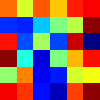
\includegraphics[width=.10\textwidth,]{BoF/desc01.png}} ;
%\draw[] (BoFi.north east) +(5pt,0) node[nameSt, label=below:(2)] (BoFii) {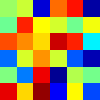
\includegraphics[width=.10\textwidth,]{BoF/desc02.png}} ;
%
%\node[nameSt, below=of dictionary, label=below:(3)] (BoFiii) {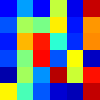
\includegraphics[width=.10\textwidth,]{BoF/desc03.png}} ;
%\node[nameSt, below=of BoFi, label=below:(4)] (BoFiv) {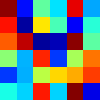
\includegraphics[width=.10\textwidth,]{BoF/desc04.png}} ;
%\node[nameSt, below=of BoFii, label=below:(5)] (BoFv) {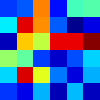
\includegraphics[width=.10\textwidth,]{BoF/desc05.png}} ;
%
%\node[nameSt, below=of BoFiii, label=below:(6)] (BoFvi) {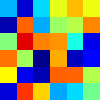
\includegraphics[width=.10\textwidth,]{BoF/desc06.png}} ;
%\node[nameSt, below=of BoFiv, label=below:(7)] (BoFvii) {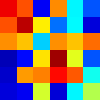
\includegraphics[width=.10\textwidth,]{BoF/desc07.png}} ;
%\node[nameSt, below=of BoFv, label=below:(8)] (BoFviii) {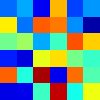
\includegraphics[width=.10\textwidth,]{BoF/desc08.png}} ;
%
%\end{tiny}

\end{tikzpicture}

\end{document}
 
%\caption{\acs{sift}-\acs{bof} descriptors qualitative analysis. (a) image example. (b) \acs{bof} descriptor building from \ac{sift} descriptors in fig.\,\ref{fig:dictionary}c. (c-f) region descriptor occurrence.{\color{red} this is a fake and the image can be redone to take less space}}
\caption{Confusion matrix results distribution represented as boxplots. The results are grouped by actual class of the samples and subdivided by the predicted label.}
\label{fig:quantitativeComparison}
\end{figure}



%The resulting space from using all the pixels as a key-point is described in figures~\ref{fig:siftMapping}, \ref{fig:siftGT} and \ref{fig:siftImg}. For displaying purposes and easier manipulation, these figures show the two dimensional representation of the \ac{sift} hyperspace obtained by projecting the 128 dimensions  of the \ac{sift} descriptors into a two dimensional space using \ac{pca}.
%Figure~\ref{fig:siftMapping}a shows this projection of the \ac{sift} space into a two dimensional space. 
%%In the figure, each sample has been colored accordingly to its \ac{gt} label. 
%In figure~\ref{fig:siftMapping}b the projected space is discretized and an occurrence study is displayed showing the distribution of the \ac{sift} descriptors present within the images. 
%%Figure~\ref{fig:siftGT} repeats the occurrence study, this time for every individual class. 
%Figure~\ref{fig:siftGT} shows the occurrence study for every class, where every different tissue type is represent by different \ac{sift} descriptors. 
%%The figure shows that different tissue types are represented by different \ac{sift} descriptors.
%Figure~\ref{fig:siftImg} qualitatively assess the description of an \ac{us} image using \ac{sift}. In fig.\,\ref{fig:siftImg}a the projected map has been arbitrarily colored, in such a manner that close projected \ac{sift} descriptors share a similar color. This coloring associated to each \ac{sift} descriptor is further used to remap the \ac{sift} descriptors extracted from the original image (see fig.\,\ref{fig:siftImg}b,c).



%Figure~\ref{fig:siftMapping}a show this projection and all the elements have been arbitrarily coded with contiguous colors, so that similar descriptors share a similar color. This coloring is further used in this study to interpret \ac{sift} images (see fig.\,\ref{fig:siftImg}). Figure~\ref{fig:siftMapping}b discretize the projected space and performs an occurrence study. Figure~\ref{fig:siftMapping}c represents the same projection however in this case the coloring is subject to the label associated to each sample. Further study of how the \ac{sift} descriptors are distributed depending on the tissue is presented in figure~\ref{fig:siftGT}. 




%Both, figure~\ref{fig:siftMapping} and \ref{fig:siftGT} qualitatively assess how 
%Figure~\ref{fig:siftImg} qualitatively assess the description of an \ac{us} image using \ac{sift}. In fig.\,\ref{fig:siftImg}a the projected map has been arbitrarily colored, in such a manner that close projected \ac{sift} descriptors share a similar color. This coloring associated to each \ac{sift} descriptor is further used to remap the \ac{sift} descriptors extracted from the original image (see fig.\,\ref{fig:siftImg}b,c).

% two \ac{sift} images by reprojecting the coloring from fig.\,\ref{fig:siftMapping}a to the \ac{sift} descriptors obtained from the example images.


\vspace{-10pt}
\section{High-level texture descriptor using Bag-of-Features (BoF) and \ac{sift} descriptors}%\acf{bof} construction from the \ac{sift} descriptors}
Texture is an area property related to spatial repetition of structures, similar statistical properties of the area or both. A technique to embed statistical properties of a low level descriptor is \ac{bof} which analyses the occurrence of a set of keywords (or key-points) within a particular region~\cite{csurka2004visual}. 

In this proposal, the words or features representing the images are \ac{sift} descriptors. In order to determine the words forming the dictionary or codebook needed to generate the \ac{bof} descriptors, the space of \ac{sift} descriptors is clustered in order to produce a hard quantification of this space. In this case, a k-means procedure with $k=36$ is used to generate the codebook. To generate the \ac{bof}-\ac{sift} feature, all the \ac{sift} descriptors are substituted for the closest \ac{sift} descriptor in the codebook. Finally the texture description from a particular area is expressed as the keywords' occurrence in this area. The descriptor is normalized so that the sum of all the occurrences is 1. 

For this application, the super-pixels of the images have been extracted using \ac{qs}%~\cite{fulkerson2012really} 
in order to extract the \ac{bof} from the obtained super-pixel regions.Figure~\ref{fig:bow} illustrates the \ac{bof}-\ac{sift} feature. On the original image, some of the super-pixels extracted have been highlighted. Figure also shows a codebook partitioning the feature space in 36 groups along with the \ac{bof} descriptors for the 8 highlighted. For the visualization of the \ac{bof} features a jet color coding has been used to represent the occurrence of each word within the codebook.




%\begin{figure}[Htbp]
%\centering
%\subfloat[]{\includegraphics[width=.2\textwidth]{fakeDict2Dmap}}~
%\subfloat[]{\includegraphics[width=.20\textwidth,]{fakeDict.png}}
%\caption{Two views of a generated codebook (dictionary) example. (a) Clusters mapped in the 2D projected \ac{sift} space. (b) Simple concatenation of the codebook for further usage visualizing super pixel's signature.}
%\label{fig:dictionaryConstruction}
%\end{figure}


%The keywords are a hard quantification of the feature space as it can be seen in figure~\ref{fig:dictionary}. Although any quantification procedure can be used, in out case a set of 36 keywords from a k-means clustering process is used (see fig.~\ref{fig:dictionary}c). Once the set of keywords determined, all the features are associated to their nearest keyword as can be observed in fig.\,\ref{fig:dictionary}. Finally the texture description from a particular area is expressed as the keywords' occurrence in this area. This process is illustrated in figure~\ref{fig:bow}.

%\begin{figure}[Htbp]
%\centering
%\subfloat[]{\includegraphics[trim=115 250 118 250,clip,width=.3\textwidth]{siftColorMap}}\,
%\subfloat[]{\includegraphics[trim=115 250 118 250,clip,width=.3\textwidth]{siftColorMap}}\,
%\subfloat[]{\includegraphics[trim=115 250 118 250,clip,width=.3\textwidth]{siftColorMap}}
%\caption{Feature space hard quantification in order to generate the set of keywords. (a) Regular sampling. (b) Aleatory sampling. (b) Clustering.{\color{red} Here should be this image but instead of smoothly change the color it should be piecewise constant (due to the quantification) first sould be like a grid and the last two like a mosaic of irregular pieces.}}
%\label{fig:dictionary}
%\end{figure}

\begin{figure}[Htbp]
\centering
% \includegraphics[trim = 91 300 100 242, clip,width=.5\textwidth]{appearance1.pdf}\\
%  \subfloat[]{\includegraphics[width=.10\textwidth,]{fakeDict.png}}\,
% \subfloat[]{\includegraphics[width=.10\textwidth,]{BoF/desc01.png}}\,
% \subfloat[]{\includegraphics[width=.10\textwidth,]{BoF/desc02.png}}\,
%  \subfloat[]{\includegraphics[width=.10\textwidth,]{BoF/desc04.png}}\,
%   \subfloat[]{\includegraphics[width=.10\textwidth,]{BoF/desc05.png}}\,
%  \subfloat[]{\includegraphics[width=.10\textwidth,]{BoF/desc03.png}}
  
 \begin{tikzpicture}
\node[anchor=south west,inner sep=0] (imgNode) at (0,0) {\includegraphics[trim = 91 300 100 242, clip,width=.635\textwidth]{appearance1.pdf}};

\tikzset{nameSt/.style=
{anchor=north west,rectangle,
node distance=10pt,
minimum width=8pt,minimum height=8pt,
inner sep=0,
}}
\begin{tiny}

\draw[] (imgNode.north east) +(5pt,0) node[nameSt, label=below:Codebook] (dictionary) {\includegraphics[width=.10\textwidth,]{dictionary/01.png}} ;
\draw[] (dictionary.north east) +(5pt,0) node[nameSt, label=below:(1)] (BoFi) {\includegraphics[width=.10\textwidth,]{dictionary/01Signatures/127.png}} ;
\draw[] (BoFi.north east) +(5pt,0) node[nameSt, label=below:(2)] (BoFii) {\includegraphics[width=.10\textwidth,]{dictionary/01Signatures/037.png}} ;

\node[nameSt, below=of dictionary, label=below:(3)] (BoFiii) {\includegraphics[width=.10\textwidth,]{dictionary/01Signatures/054.png}} ;
\node[nameSt, below=of BoFi, label=below:(4)] (BoFiv) {\includegraphics[width=.10\textwidth,]{dictionary/01Signatures/118.png}} ;
\node[nameSt, below=of BoFii, label=below:(5)] (BoFv) {\includegraphics[width=.10\textwidth,]{dictionary/01Signatures/160.png}} ;

\node[nameSt, below=of BoFiii, label=below:(6)] (BoFvi) {\includegraphics[width=.10\textwidth,]{dictionary/01Signatures/061.png}} ;
\node[nameSt, below=of BoFiv, label=below:(7)] (BoFvii) {\includegraphics[width=.10\textwidth,]{dictionary/01Signatures/077.png}} ;
\node[nameSt, below=of BoFv, label=below:(8)] (BoFviii) {\includegraphics[width=.10\textwidth,]{dictionary/01Signatures/043.png}} ;

\end{tiny}

\end{tikzpicture}
 
%\caption{\acs{sift}-\acs{bof} descriptors qualitative analysis. (a) image example. (b) \acs{bof} descriptor building from \ac{sift} descriptors in fig.\,\ref{fig:dictionary}c. (c-f) region descriptor occurrence.{\color{red} this is a fake and the image can be redone to take less space}}
\caption{\acs{sift}-\acs{bof} descriptors qualitative analysis. (Left) image example. (Right) Dictionary representation colored using the location of the keypoint location in fig.\,\ref{fig:siftMapping}a space. (1-8) Occurrence of the dictionary's key-points associated to each region highlighted in the original image.}
\label{fig:bow}
\end{figure}

In order to quantitatively assess the performance of \ac{sift} embedded within in a high-level feature descriptor such as \ac{bof}, a dataset of super-pixels with its associated \ac{gt} and \ac{bof}-\ac{sift} descriptor has been build up. In order for the super-pixels to be eligible it has been set up that the superpixel should be larger than 50 pixels and be fully contained within the same \ac{gt} label. This second constrain has been relaxed for skin and rib classes allowing super-pixels with $75\%$ label contained to be eligible. The study has been carried out only for all the main classes, thus excluding background and boundary classes. To carry out the evaluation $20$ folds of $8$ super-pixels (one per class) have been selected forming a set of $152$ samples for training and $8$ samples for testing at each round. The experiments have been repeated under the same conditions with $3$ different codebooks in order to take into account the variability introduced by the codebook building. As for the case of low-level texture description the experiments have been duplicated using intensity for comparison purposes. The classification has been carried out using \ac{svm}. The \ac{tpr} results achieved are $29\pm3.6\%$ for the case of intensity and $33.5\pm2.3\%$ for the case of \ac{sift}, showing their similar performance and the improvement from using high-level texture descriptor over the low-level texture descriptor.

\vspace{-10pt}

\section{Conclusion} 
\vspace{-3pt}
The present study was designed to explore the usage of \ac{sift} feature space as a texture for characterizing the different tissues present in a breast \ac{us} image. During the study, \ac{sift} information have been used both as a low-level texture descriptor and encoded within a high-level texture descriptor using \ac{bof}. When comparing the performance of using the \ac{sift} space with the intensity to characterize tissues both spaces reach similar results. 

One of the limitations of the study here presented is that in order to get a graphical representation of the \ac{sift} space, the 128 dimensions have been reduced to two compromising its performance. 

The fact that despite all this limitations, \ac{sift} and intensity spaces, still produce similar results encourage further studies on using \ac{sift}.

\vspace{-5pt}
%\newpage
%\bibliographystyle{splncs}
\bibliographystyle{plain}
\bibliography{bibliografiaNew}

\end{document}

